% ============================================================================
%  BÁO CÁO ĐỒ ÁN MÔN HỌC — CS221 Xử lý ngôn ngữ tự nhiên
%  Đề tài: Khảo sát và đánh giá hiệu năng các mô hình Transformer tiền huấn luyện
%          trong bài toán đọc hiểu văn bản và trả lời câu hỏi tiếng Việt
%  Biên dịch:  python scripts/make_report_numbers.py && latexmk -xelatex main.tex
%  Mọi con số kết quả đến từ generated/*.tex, sinh từ results/*.json — không gõ tay.
% ============================================================================
\documentclass[12pt,a4paper]{article}

% ---------- Font & ngôn ngữ ----------
\usepackage{fontspec}
\setmainfont{lmroman12-regular.otf}[
  BoldFont       = lmroman12-bold.otf,
  ItalicFont     = lmroman12-italic.otf,
  BoldItalicFont = lmroman10-bolditalic.otf,
  SmallCapsFont  = lmromancaps10-regular.otf]
\setsansfont{lmsans12-regular.otf}[BoldFont = lmsans10-bold.otf]
\setmonofont{lmmono10-regular.otf}[Scale=0.95,BoldFont=lmmonolt10-bold.otf]
\usepackage[vietnamese]{babel}

% ---------- Trang ----------
\usepackage[a4paper,top=2.5cm,bottom=2.5cm,left=3cm,right=2.2cm,headheight=15pt]{geometry}
\usepackage{setspace}
\setstretch{1.12}
\setlength{\parskip}{0.25em}
\usepackage{microtype}
\setlength{\emergencystretch}{3em}
\usepackage{fancyhdr}
\usepackage{titlesec}
\usepackage{enumitem}
\setlist{itemsep=0.15em,topsep=0.3em}

% ---------- Toán, bảng, hình ----------
\usepackage{amsmath,amssymb}
\usepackage{booktabs,tabularx,multirow,array,longtable}
\usepackage{graphicx}
\usepackage[table]{xcolor}
\usepackage{caption}
\captionsetup{font=small,labelfont=bf,labelsep=period,justification=centering}
\usepackage{subcaption}
\usepackage{float}
\usepackage[section]{placeins}
\usepackage{pifont}
\usepackage{tikz}
\usetikzlibrary{arrows.meta,positioning,fit,backgrounds,calc,shapes.geometric,decorations.pathreplacing}
\usepackage[most]{tcolorbox}
\usepackage{listings}
\usepackage[ruled,vlined,linesnumbered]{algorithm2e}
\usepackage{hyperref}
\hypersetup{colorlinks=true,linkcolor=black,citecolor=uitblue,urlcolor=uitblue,
  pdftitle={CS221 - Danh gia Transformer cho doc hieu tieng Viet},
  pdfauthor={Nhom do an CS221}}

% ---------- Màu & hộp nhấn mạnh ----------
\definecolor{uitblue}{HTML}{2F5BB7}
\definecolor{softgray}{HTML}{F4F5F7}
\definecolor{warnorange}{HTML}{B85C00}
\definecolor{okgreen}{HTML}{2E7D32}
\definecolor{badred}{HTML}{B3261E}
\newtcolorbox{keybox}[1][]{enhanced,breakable,colback=softgray,colframe=uitblue,
  boxrule=0pt,leftrule=3pt,arc=0pt,left=8pt,right=8pt,top=5pt,bottom=5pt,#1}
\newtcolorbox{warnbox}[1][]{enhanced,breakable,colback=orange!6,colframe=warnorange,
  boxrule=0pt,leftrule=3pt,arc=0pt,left=8pt,right=8pt,top=5pt,bottom=5pt,#1}

\lstset{basicstyle=\ttfamily\footnotesize,columns=fullflexible,keepspaces=true,
  frame=single,rulecolor=\color{black!20},backgroundcolor=\color{softgray},
  numbers=none,breaklines=true,showstringspaces=false,
  keywordstyle=\color{uitblue}\bfseries,commentstyle=\color{black!55}\itshape,
  stringstyle=\color{okgreen},xleftmargin=4pt,xrightmargin=4pt,aboveskip=6pt,belowskip=6pt}

% ---------- Tiêu đề mục ----------
\titleformat{\section}{\normalfont\Large\bfseries}{\thesection}{0.8em}{}
\titleformat{\subsection}{\normalfont\large\bfseries}{\thesubsection}{0.8em}{}
\titleformat{\subsubsection}{\normalfont\normalsize\bfseries}{\thesubsubsection}{0.8em}{}
\titlespacing*{\section}{0pt}{0pt}{1.2em}
\titlespacing*{\subsection}{0pt}{1.1em}{0.5em}
\titlespacing*{\subsubsection}{0pt}{0.9em}{0.3em}
\setcounter{secnumdepth}{3}
\setcounter{tocdepth}{2}

% ---------- Thuật ngữ trong algorithm2e ----------
\SetKwInput{KwIn}{Đầu vào}
\SetKwInput{KwOut}{Đầu ra}
\SetAlgorithmName{Thuật toán}{thuật toán}{Danh sách thuật toán}
\SetKwFor{ForEach}{với mỗi}{thực hiện}{hết}
\SetKwIF{If}{ElseIf}{Else}{nếu}{thì}{ngược lại nếu}{ngược lại}{hết}
\SetKw{Return}{trả về}
\SetKw{Continue}{bỏ qua}

% ---------- Tiện ích ----------
\newcommand{\code}[1]{\texttt{#1}}
\newcommand{\yes}{\textcolor{okgreen}{\ding{51}}}
\newcommand{\no}{\textcolor{badred}{\ding{55}}}
\newcommand{\unk}{\textcolor{black!55}{\ding{110}}}
\newcolumntype{R}{>{\raggedleft\arraybackslash}X}
\newcolumntype{L}{>{\raggedright\arraybackslash}X}
\newcolumntype{C}{>{\centering\arraybackslash}X}

% ---------- Tên gọi tiếng Việt ----------
\addto\captionsvietnamese{%
  \renewcommand{\contentsname}{Mục lục}%
  \renewcommand{\listfigurename}{Danh sách hình vẽ}%
  \renewcommand{\listtablename}{Danh sách bảng}%
  \renewcommand{\refname}{Tài liệu tham khảo}%
  \renewcommand{\figurename}{Hình}%
  \renewcommand{\tablename}{Bảng}}

% ---------- Header / footer ----------
\pagestyle{fancy}
\fancyhf{}
\fancyhead[L]{\small\color{black!60}CS221 --- Xử lý ngôn ngữ tự nhiên}
\fancyhead[R]{\small\color{black!60}Transformer cho đọc hiểu tiếng Việt}
\fancyfoot[C]{\small\thepage}
\renewcommand{\headrulewidth}{0.4pt}
\fancypagestyle{plain}{\fancyhf{}\fancyfoot[C]{\small\thepage}\renewcommand{\headrulewidth}{0pt}}


% Số liệu sinh tự động từ results/*.json (scripts/make_report_numbers.py)
% SINH TỰ ĐỘNG bởi scripts/make_report_numbers.py — KHÔNG SỬA TAY
\providecommand{\missing}{\textcolor{badred}{\textbf{??}}}
\newcommand{\NTrain}{28.454}
\newcommand{\NTrainCtx}{4.101}
\newcommand{\NTrainImp}{9.216}
\newcommand{\PctTrainImp}{32{,}39}
\newcommand{\NTrainAns}{19.238}
\newcommand{\NVal}{3.814}
\newcommand{\NValCtx}{557}
\newcommand{\NValImp}{1.161}
\newcommand{\PctValImp}{30{,}44}
\newcommand{\NValAns}{2.653}
\newcommand{\NFit}{27.049}
\newcommand{\NFitCtx}{3.896}
\newcommand{\NFitImp}{8.773}
\newcommand{\PctFitImp}{32{,}43}
\newcommand{\NFitAns}{18.276}
\newcommand{\NDev}{1.405}
\newcommand{\NDevCtx}{205}
\newcommand{\NDevImp}{443}
\newcommand{\PctDevImp}{31{,}53}
\newcommand{\NDevAns}{962}
\newcommand{\SegN}{2.653}
\newcommand{\SegAligned}{2.620}
\newcommand{\SegMis}{33}
\newcommand{\SegStartCut}{13}
\newcommand{\SegEndCut}{20}
\newcommand{\SegCtx}{557}
\newcommand{\SegMisPct}{1{,}24}
\newcommand{\SegOracle}{99{,}25}
\newcommand{\SegOracleMis}{39{,}39}
\newcommand{\SegAlignedPct}{98{,}76}
\newcommand{\SegCeilingLoss}{0{,}75}
\newcommand{\SegCtxCoverage}{100{,}00}
\newcommand{\MisPeriod}{13}
\newcommand{\MisMerge}{12}
\newcommand{\MisCompound}{3}
\newcommand{\MisAnnot}{5}
\newcommand{\AuditN}{250}
\newcommand{\AuditAns}{120}
\newcommand{\AuditAnsInCtx}{15}
\newcommand{\AuditOffsetOK}{6}
\newcommand{\AuditValid}{145}
\newcommand{\AuditCtx}{5}
\newcommand{\AuditFlat}{120}
\newcommand{\AuditCombined}{370}
\newcommand{\AuditTrainOverlap}{0}
\newcommand{\AuditEOneValid}{14}
\newcommand{\AuditEOneAns}{41}
\newcommand{\AuditEOneAnsInCtx}{5}
\newcommand{\AuditEOneDistinctQ}{21}
\newcommand{\AuditETwoValid}{17}
\newcommand{\AuditETwoAns}{35}
\newcommand{\AuditETwoAnsInCtx}{2}
\newcommand{\AuditETwoDistinctQ}{28}
\newcommand{\AuditEThreeValid}{50}
\newcommand{\AuditEThreeAns}{0}
\newcommand{\AuditEThreeAnsInCtx}{0}
\newcommand{\AuditEThreeDistinctQ}{14}
\newcommand{\AuditEFourValid}{18}
\newcommand{\AuditEFourAns}{37}
\newcommand{\AuditEFourAnsInCtx}{5}
\newcommand{\AuditEFourDistinctQ}{13}
\newcommand{\AuditEFiveValid}{46}
\newcommand{\AuditEFiveAns}{7}
\newcommand{\AuditEFiveAnsInCtx}{3}
\newcommand{\AuditEFiveDistinctQ}{8}
\newcommand{\AbstainEM}{30{,}44}
\newcommand{\AbstainFone}{30{,}44}
\newcommand{\AbstainAnsEM}{0{,}00}
\newcommand{\AbstainAnsFone}{0{,}00}
\newcommand{\AbstainImpEM}{100{,}00}
\newcommand{\AbstainLat}{0{,}00}
\newcommand{\AbstainStressEM}{52{,}00}
\newcommand{\AbstainAbsRate}{100{,}00}
\newcommand{\AbstainAbsPrec}{30{,}44}
\newcommand{\AbstainAbsRec}{100{,}00}
\newcommand{\AbstainTrapN}{0}
\newcommand{\AbstainTrapHit}{0}
\newcommand{\AbstainTrapPct}{\missing{}}
\newcommand{\AbstainAlEM}{0{,}00}
\newcommand{\AbstainMisEM}{0{,}00}
\newcommand{\AbstainMisFone}{0{,}00}
\newcommand{\AbstainNErr}{2.653}
\newcommand{\AbstainErrBoundary}{0}
\newcommand{\AbstainErrBoundaryPct}{0{,}00}
\newcommand{\AbstainAnsweredAns}{0}
\newcommand{\AbstainBoundaryRate}{\missing{}}
\newcommand{\AbstainErrFalseAbs}{2.653}
\newcommand{\AbstainErrFalseAbsPct}{100{,}00}
\newcommand{\AbstainErrFalseAns}{0}
\newcommand{\AbstainErrFalseAnsPct}{0{,}00}
\newcommand{\AbstainErrWrong}{0}
\newcommand{\AbstainErrWrongPct}{0{,}00}
\newcommand{\AbstainErrSuper}{0}
\newcommand{\AbstainErrSuperPct}{0{,}00}
\newcommand{\AbstainErrSub}{0}
\newcommand{\AbstainErrSubPct}{0{,}00}
\newcommand{\AbstainErrOverlap}{0}
\newcommand{\AbstainErrOverlapPct}{0{,}00}
\newcommand{\TfidfEM}{1{,}05}
\newcommand{\TfidfFone}{22{,}11}
\newcommand{\TfidfAnsEM}{1{,}51}
\newcommand{\TfidfAnsFone}{31{,}79}
\newcommand{\TfidfImpEM}{0{,}00}
\newcommand{\TfidfLat}{0{,}86}
\newcommand{\TfidfStressEM}{0{,}00}
\newcommand{\TfidfAbsRate}{0{,}00}
\newcommand{\TfidfAbsPrec}{0{,}00}
\newcommand{\TfidfAbsRec}{0{,}00}
\newcommand{\TfidfTrapN}{1.161}
\newcommand{\TfidfTrapHit}{16}
\newcommand{\TfidfTrapPct}{1{,}38}
\newcommand{\TfidfAlEM}{1{,}53}
\newcommand{\TfidfMisEM}{0{,}00}
\newcommand{\TfidfMisFone}{25{,}91}
\newcommand{\TfidfNErr}{3.774}
\newcommand{\TfidfErrBoundary}{2.397}
\newcommand{\TfidfErrBoundaryPct}{63{,}51}
\newcommand{\TfidfAnsweredAns}{2.653}
\newcommand{\TfidfBoundaryRate}{90{,}35}
\newcommand{\TfidfErrFalseAbs}{0}
\newcommand{\TfidfErrFalseAbsPct}{0{,}00}
\newcommand{\TfidfErrFalseAns}{1.161}
\newcommand{\TfidfErrFalseAnsPct}{30{,}76}
\newcommand{\TfidfErrWrong}{216}
\newcommand{\TfidfErrWrongPct}{5{,}72}
\newcommand{\TfidfErrSuper}{1.938}
\newcommand{\TfidfErrSuperPct}{51{,}35}
\newcommand{\TfidfErrSub}{2}
\newcommand{\TfidfErrSubPct}{0{,}05}
\newcommand{\TfidfErrOverlap}{457}
\newcommand{\TfidfErrOverlapPct}{12{,}11}
\newcommand{\XlmrEM}{52{,}49}
\newcommand{\XlmrFone}{61{,}32}
\newcommand{\XlmrAnsEM}{52{,}02}
\newcommand{\XlmrAnsFone}{64{,}71}
\newcommand{\XlmrImpEM}{53{,}57}
\newcommand{\XlmrLat}{15{,}48}
\newcommand{\XlmrStressEM}{51{,}20}
\newcommand{\XlmrAbsRate}{32{,}96}
\newcommand{\XlmrAbsPrec}{49{,}48}
\newcommand{\XlmrAbsRec}{53{,}57}
\newcommand{\XlmrTrapN}{539}
\newcommand{\XlmrTrapHit}{277}
\newcommand{\XlmrTrapPct}{51{,}39}
\newcommand{\XlmrAlEM}{52{,}10}
\newcommand{\XlmrMisEM}{45{,}45}
\newcommand{\XlmrMisFone}{56{,}12}
\newcommand{\XlmrNErr}{1.812}
\newcommand{\XlmrErrBoundary}{542}
\newcommand{\XlmrErrBoundaryPct}{29{,}91}
\newcommand{\XlmrAnsweredAns}{2.018}
\newcommand{\XlmrBoundaryRate}{26{,}86}
\newcommand{\XlmrErrFalseAbs}{635}
\newcommand{\XlmrErrFalseAbsPct}{35{,}04}
\newcommand{\XlmrErrFalseAns}{539}
\newcommand{\XlmrErrFalseAnsPct}{29{,}75}
\newcommand{\XlmrErrWrong}{96}
\newcommand{\XlmrErrWrongPct}{5{,}30}
\newcommand{\XlmrErrSuper}{258}
\newcommand{\XlmrErrSuperPct}{14{,}24}
\newcommand{\XlmrErrSub}{181}
\newcommand{\XlmrErrSubPct}{9{,}99}
\newcommand{\XlmrErrOverlap}{103}
\newcommand{\XlmrErrOverlapPct}{5{,}68}
\newcommand{\PhobertEM}{51{,}36}
\newcommand{\PhobertFone}{63{,}10}
\newcommand{\PhobertAnsEM}{66{,}91}
\newcommand{\PhobertAnsFone}{83{,}77}
\newcommand{\PhobertImpEM}{15{,}85}
\newcommand{\PhobertLat}{13{,}60}
\newcommand{\PhobertStressEM}{48{,}00}
\newcommand{\PhobertAbsRate}{5{,}66}
\newcommand{\PhobertAbsPrec}{85{,}19}
\newcommand{\PhobertAbsRec}{15{,}85}
\newcommand{\PhobertTrapN}{977}
\newcommand{\PhobertTrapHit}{443}
\newcommand{\PhobertTrapPct}{45{,}34}
\newcommand{\PhobertAlEM}{67{,}37}
\newcommand{\PhobertMisEM}{30{,}30}
\newcommand{\PhobertMisFone}{70{,}96}
\newcommand{\PhobertNErr}{1.855}
\newcommand{\PhobertErrBoundary}{724}
\newcommand{\PhobertErrBoundaryPct}{39{,}03}
\newcommand{\PhobertAnsweredAns}{2.621}
\newcommand{\PhobertBoundaryRate}{27{,}62}
\newcommand{\PhobertErrFalseAbs}{32}
\newcommand{\PhobertErrFalseAbsPct}{1{,}73}
\newcommand{\PhobertErrFalseAns}{977}
\newcommand{\PhobertErrFalseAnsPct}{52{,}67}
\newcommand{\PhobertErrWrong}{122}
\newcommand{\PhobertErrWrongPct}{6{,}58}
\newcommand{\PhobertErrSuper}{354}
\newcommand{\PhobertErrSuperPct}{19{,}08}
\newcommand{\PhobertErrSub}{223}
\newcommand{\PhobertErrSubPct}{12{,}02}
\newcommand{\PhobertErrOverlap}{147}
\newcommand{\PhobertErrOverlapPct}{7{,}92}
\newcommand{\NLenOne}{657}
\newcommand{\NLenThree}{597}
\newcommand{\NLenSix}{540}
\newcommand{\NLenEleven}{859}
\newcommand{\PairN}{3.814}
\newcommand{\PairDiff}{-1{,}13}
\newcommand{\PairLo}{-2{,}88}
\newcommand{\PairHi}{0{,}60}
\newcommand{\PairArtLo}{-3{,}53}
\newcommand{\PairArtHi}{0{,}91}
\newcommand{\PairP}{0{,}223}
\newcommand{\PairOnlyP}{573}
\newcommand{\PairOnlyX}{616}
\newcommand{\PairBoth}{1.386}
\newcommand{\PairNeither}{1.239}
\newcommand{\PairAnsN}{2.653}
\newcommand{\PairAnsDiff}{14{,}89}
\newcommand{\PairAnsLo}{13{,}08}
\newcommand{\PairAnsHi}{16{,}77}
\newcommand{\PairAnsArtLo}{11{,}82}
\newcommand{\PairAnsArtHi}{17{,}60}
\newcommand{\PairAnsP}{$<$\,0{,}001}
\newcommand{\PairAnsOnlyP}{544}
\newcommand{\PairAnsOnlyX}{149}
\newcommand{\PairAnsBoth}{1.231}
\newcommand{\PairAnsNeither}{729}
\newcommand{\PairImpN}{1.161}
\newcommand{\PairImpDiff}{-37{,}73}
\newcommand{\PairImpLo}{-40{,}83}
\newcommand{\PairImpHi}{-34{,}63}
\newcommand{\PairImpArtLo}{-43{,}81}
\newcommand{\PairImpArtHi}{-32{,}28}
\newcommand{\PairImpP}{$<$\,0{,}001}
\newcommand{\PairImpOnlyP}{29}
\newcommand{\PairImpOnlyX}{467}
\newcommand{\PairImpBoth}{155}
\newcommand{\PairImpNeither}{510}
\newcommand{\PairMisN}{33}
\newcommand{\PairMisDiff}{-15{,}15}
\newcommand{\PairMisLo}{-33{,}33}
\newcommand{\PairMisHi}{3{,}03}
\newcommand{\PairMisArtLo}{\missing{}}
\newcommand{\PairMisArtHi}{\missing{}}
\newcommand{\PairMisP}{0{,}180}
\newcommand{\PairMisOnlyP}{2}
\newcommand{\PairMisOnlyX}{7}
\newcommand{\PairMisBoth}{8}
\newcommand{\PairMisNeither}{16}
\newcommand{\XlmrBestEpoch}{3}
\newcommand{\XlmrMaxLen}{384}
\newcommand{\XlmrStride}{128}
\newcommand{\XlmrEpochs}{3}
\newcommand{\XlmrTrainMin}{106}
\newcommand{\PhobertRunABestEpoch}{3}
\newcommand{\PhobertRunAMaxLen}{256}
\newcommand{\PhobertRunAStride}{96}
\newcommand{\PhobertRunAEpochs}{3}
\newcommand{\PhobertRunATrainMin}{67}
\newcommand{\PhobertRunBBestEpoch}{2}
\newcommand{\PhobertRunBMaxLen}{256}
\newcommand{\PhobertRunBStride}{96}
\newcommand{\PhobertRunBEpochs}{3}
\newcommand{\PhobertRunBTrainMin}{68}
\newcommand{\PhobertRunCBestEpoch}{3}
\newcommand{\PhobertRunCMaxLen}{256}
\newcommand{\PhobertRunCStride}{96}
\newcommand{\PhobertRunCEpochs}{3}
\newcommand{\PhobertRunCTrainMin}{68}
\newcommand{\PhobertRunADevFone}{60{,}61}
\newcommand{\PhobertRunAFullDevFone}{61{,}16}
\newcommand{\PhobertRunAStable}{sụp đổ}
\newcommand{\PhobertRunAEM}{51{,}36}
\newcommand{\PhobertRunAAnsEM}{66{,}91}
\newcommand{\PhobertRunAImpEM}{15{,}85}
\newcommand{\PhobertRunAAbsRate}{5{,}66}
\newcommand{\PhobertRunBDevFone}{58{,}36}
\newcommand{\PhobertRunBFullDevFone}{57{,}74}
\newcommand{\PhobertRunBStable}{sụp đổ}
\newcommand{\PhobertRunBEM}{49{,}55}
\newcommand{\PhobertRunBAnsEM}{65{,}21}
\newcommand{\PhobertRunBImpEM}{13{,}78}
\newcommand{\PhobertRunBAbsRate}{5{,}43}
\newcommand{\PhobertRunCDevFone}{59{,}24}
\newcommand{\PhobertRunCFullDevFone}{60{,}56}
\newcommand{\PhobertRunCStable}{ổn định}
\newcommand{\PhobertRunCEM}{54{,}09}
\newcommand{\PhobertRunCAnsEM}{57{,}86}
\newcommand{\PhobertRunCImpEM}{45{,}48}
\newcommand{\PhobertRunCAbsRate}{23{,}75}
\newcommand{\PhobertPrimaryLabel}{PhoBERT, lr $3\cdot10^{-5}$}
\newcommand{\ProbeXlmrClsFrac}{36{,}56}
\newcommand{\ProbeXlmrClsOne}{0{,}74}
\newcommand{\ProbeXlmrSpanOne}{1{,}59}
\newcommand{\ProbeXlmrClsTwo}{0{,}61}
\newcommand{\ProbeXlmrSpanTwo}{1{,}18}
\newcommand{\ProbeXlmrClsThree}{0{,}72}
\newcommand{\ProbeXlmrSpanThree}{0{,}88}
\newcommand{\ProbePhobertRunAClsFrac}{39{,}62}
\newcommand{\ProbePhobertRunAClsOne}{0{,}56}
\newcommand{\ProbePhobertRunASpanOne}{1{,}35}
\newcommand{\ProbePhobertRunAClsTwo}{4{,}18}
\newcommand{\ProbePhobertRunASpanTwo}{0{,}88}
\newcommand{\ProbePhobertRunAClsThree}{4{,}28}
\newcommand{\ProbePhobertRunASpanThree}{0{,}63}
\newcommand{\ProbePhobertRunBClsFrac}{39{,}62}
\newcommand{\ProbePhobertRunBClsOne}{0{,}58}
\newcommand{\ProbePhobertRunBSpanOne}{1{,}50}
\newcommand{\ProbePhobertRunBClsTwo}{4{,}33}
\newcommand{\ProbePhobertRunBSpanTwo}{1{,}02}
\newcommand{\ProbePhobertRunBClsThree}{4{,}42}
\newcommand{\ProbePhobertRunBSpanThree}{0{,}82}
\newcommand{\ThrXlmrTau}{-0{,}47}
\newcommand{\ThrXlmrDevFone}{61{,}29}
\newcommand{\ThrXlmrDevFoneZero}{60{,}78}
\newcommand{\ThrXlmrDevAbsRate}{25{,}48}
\newcommand{\ThrXlmrEMZero}{52{,}49}
\newcommand{\ThrXlmrEM}{52{,}49}
\newcommand{\ThrXlmrFoneZero}{61{,}32}
\newcommand{\ThrXlmrFone}{61{,}99}
\newcommand{\ThrXlmrAnsEMZero}{52{,}02}
\newcommand{\ThrXlmrAnsEM}{54{,}62}
\newcommand{\ThrXlmrImpEMZero}{53{,}57}
\newcommand{\ThrXlmrImpEM}{47{,}63}
\newcommand{\ThrXlmrAbsRateZero}{32{,}96}
\newcommand{\ThrXlmrAbsRate}{27{,}77}
\newcommand{\ThrPhobertRunATau}{7{,}86}
\newcommand{\ThrPhobertRunADevFone}{68{,}02}
\newcommand{\ThrPhobertRunADevFoneZero}{61{,}16}
\newcommand{\ThrPhobertRunADevAbsRate}{27{,}54}
\newcommand{\ThrPhobertRunAEMZero}{51{,}36}
\newcommand{\ThrPhobertRunAEM}{58{,}31}
\newcommand{\ThrPhobertRunAFoneZero}{63{,}10}
\newcommand{\ThrPhobertRunAFone}{68{,}54}
\newcommand{\ThrPhobertRunAAnsEMZero}{66{,}91}
\newcommand{\ThrPhobertRunAAnsEM}{60{,}57}
\newcommand{\ThrPhobertRunAImpEMZero}{15{,}85}
\newcommand{\ThrPhobertRunAImpEM}{53{,}14}
\newcommand{\ThrPhobertRunAAbsRateZero}{5{,}66}
\newcommand{\ThrPhobertRunAAbsRate}{24{,}96}
\newcommand{\ThrPhobertRunBTau}{8{,}03}
\newcommand{\ThrPhobertRunBDevFone}{63{,}44}
\newcommand{\ThrPhobertRunBDevFoneZero}{57{,}74}
\newcommand{\ThrPhobertRunBDevAbsRate}{29{,}32}
\newcommand{\ThrPhobertRunBEMZero}{49{,}55}
\newcommand{\ThrPhobertRunBEM}{56{,}27}
\newcommand{\ThrPhobertRunBFoneZero}{61{,}13}
\newcommand{\ThrPhobertRunBFone}{65{,}37}
\newcommand{\ThrPhobertRunBAnsEMZero}{65{,}21}
\newcommand{\ThrPhobertRunBAnsEM}{57{,}22}
\newcommand{\ThrPhobertRunBImpEMZero}{13{,}78}
\newcommand{\ThrPhobertRunBImpEM}{54{,}09}
\newcommand{\ThrPhobertRunBAbsRateZero}{5{,}43}
\newcommand{\ThrPhobertRunBAbsRate}{29{,}05}
\newcommand{\ThrPhobertRunCTau}{\missing{}}
\newcommand{\ThrPhobertRunCDevFone}{\missing{}}
\newcommand{\ThrPhobertRunCDevFoneZero}{\missing{}}
\newcommand{\ThrPhobertRunCDevAbsRate}{\missing{}}
\newcommand{\ThrPhobertRunCEMZero}{\missing{}}
\newcommand{\ThrPhobertRunCEM}{\missing{}}
\newcommand{\ThrPhobertRunCFoneZero}{\missing{}}
\newcommand{\ThrPhobertRunCFone}{\missing{}}
\newcommand{\ThrPhobertRunCAnsEMZero}{\missing{}}
\newcommand{\ThrPhobertRunCAnsEM}{\missing{}}
\newcommand{\ThrPhobertRunCImpEMZero}{\missing{}}
\newcommand{\ThrPhobertRunCImpEM}{\missing{}}
\newcommand{\ThrPhobertRunCAbsRateZero}{\missing{}}
\newcommand{\ThrPhobertRunCAbsRate}{\missing{}}
\newcommand{\ThrPhobertEM}{58{,}31}
\newcommand{\ThrPhobertEMZero}{51{,}36}
\newcommand{\ThrPhobertFone}{68{,}54}
\newcommand{\ThrPhobertFoneZero}{63{,}10}
\newcommand{\ThrPhobertAnsEM}{60{,}57}
\newcommand{\ThrPhobertAnsEMZero}{66{,}91}
\newcommand{\ThrPhobertImpEM}{53{,}14}
\newcommand{\ThrPhobertImpEMZero}{15{,}85}
\newcommand{\ThrPhobertAbsRate}{24{,}96}
\newcommand{\ThrPhobertAbsRateZero}{5{,}66}
\newcommand{\ThrPhobertTau}{7{,}86}
\newcommand{\BothN}{2.011}
\newcommand{\BothPhobert}{72{,}55}
\newcommand{\BothXlmr}{68{,}42}
\newcommand{\BothGap}{4{,}13}
\newcommand{\BothTunedN}{1.971}
\newcommand{\BothTunedPhobert}{72{,}15}
\newcommand{\BothTunedXlmr}{68{,}09}
\newcommand{\BothTunedGap}{4{,}06}
\newcommand{\PairTDiff}{5{,}82}
\newcommand{\PairTArtLo}{3{,}60}
\newcommand{\PairTArtHi}{7{,}72}
\newcommand{\PairTP}{$<$\,0{,}001}
\newcommand{\PairTAnsDiff}{5{,}96}
\newcommand{\PairTAnsArtLo}{3{,}77}
\newcommand{\PairTAnsArtHi}{7{,}80}
\newcommand{\PairTAnsP}{$<$\,0{,}001}
\newcommand{\PairTImpDiff}{5{,}51}
\newcommand{\PairTImpArtLo}{0{,}08}
\newcommand{\PairTImpArtHi}{11{,}27}
\newcommand{\PairTImpP}{0{,}001}
\newcommand{\DevEpochOneEM}{46{,}76}
\newcommand{\DevEpochOneFone}{60{,}59}
\newcommand{\DevEpochOneAbsRate}{37{,}86}
\newcommand{\DevRunAEM}{44{,}34}
\newcommand{\DevRunAFone}{61{,}16}
\newcommand{\DevRunAAbsRate}{7{,}47}
\newcommand{\DevRunBEM}{40{,}57}
\newcommand{\DevRunBFone}{57{,}74}
\newcommand{\DevRunBAbsRate}{5{,}77}
\newcommand{\DevRunCEM}{44{,}20}
\newcommand{\DevRunCFone}{60{,}56}
\newcommand{\DevRunCAbsRate}{20{,}93}
\newcommand{\DevXlmrEM}{48{,}19}
\newcommand{\DevXlmrFone}{60{,}78}
\newcommand{\DevXlmrAbsRate}{32{,}31}
\newcommand{\NDevFull}{1.405}
\newcommand{\ScanPhobertFeatures}{31.039}
\newcommand{\ScanPhobertViolations}{0}
\newcommand{\ScanPhobertMismatchPct}{1{,}66}
\newcommand{\ScanPhobertClsFrac}{39{,}14}
\newcommand{\ScanXlmrFeatures}{28.887}
\newcommand{\ScanXlmrViolations}{0}
\newcommand{\ScanXlmrMismatchPct}{0{,}50}
\newcommand{\ScanXlmrClsFrac}{35{,}96}
\newcommand{\ResumeHighStable}{sụp đổ}
\newcommand{\ResumeHighMaxRise}{1{,}50}
\newcommand{\ResumeHighFirstViolation}{549}
\newcommand{\ResumeHighNSpikes}{9}
\newcommand{\ResumeHighMaxSpike}{12.880}
\newcommand{\ResumeHighMaxSpikeStep}{570}
\newcommand{\ResumeHighFirstSpikeStep}{522}
\newcommand{\ResumeHighClsStart}{0{,}71}
\newcommand{\ResumeHighClsEnd}{4{,}35}
\newcommand{\ResumeHighSpanEnd}{1{,}34}
\newcommand{\ResumeLowStable}{ổn định}
\newcommand{\ResumeLowMaxRise}{0{,}04}
\newcommand{\ResumeLowFirstViolation}{\missing{}}
\newcommand{\ResumeLowNSpikes}{0}
\newcommand{\ResumeLowMaxSpike}{0}
\newcommand{\ResumeLowMaxSpikeStep}{\missing{}}
\newcommand{\ResumeLowFirstSpikeStep}{\missing{}}
\newcommand{\ResumeLowClsStart}{0{,}69}
\newcommand{\ResumeLowClsEnd}{0{,}71}
\newcommand{\ResumeLowSpanEnd}{1{,}31}
\newcommand{\PubBaseFone}{63{,}03}
\newcommand{\PubBaseEM}{53{,}55}
\newcommand{\PubBestFone}{84{,}24}
\newcommand{\PubBestEM}{77{,}99}
\newcommand{\PubMeanFone}{70{,}70}
\newcommand{\PubMeanEM}{61{,}13}
\newcommand{\PubHumanFone}{87{,}34}
\newcommand{\PubHumanEM}{82{,}85}
\newcommand{\PubPrivPhobertLargeFone}{70{,}10}
\newcommand{\PubPrivWinnerFone}{77{,}24}
\newcommand{\SeedXlmrSEM}{52{,}49}
\newcommand{\SeedXlmrSFone}{61{,}32}
\newcommand{\SeedXlmrSTunedFone}{61{,}99}
\newcommand{\SeedXlmrSThirteenEM}{53{,}64}
\newcommand{\SeedXlmrSThirteenFone}{62{,}18}
\newcommand{\SeedXlmrSThirteenTunedFone}{\missing{}}
\newcommand{\SeedXlmrTwoFiftySixEM}{\missing{}}
\newcommand{\SeedXlmrTwoFiftySixFone}{\missing{}}
\newcommand{\SeedXlmrTwoFiftySixTunedFone}{\missing{}}
\newcommand{\SeedPhobertSEM}{51{,}36}
\newcommand{\SeedPhobertSFone}{63{,}10}
\newcommand{\SeedPhobertSTunedFone}{68{,}54}
\newcommand{\SeedPhobertSThirteenEM}{\missing{}}
\newcommand{\SeedPhobertSThirteenFone}{\missing{}}
\newcommand{\SeedPhobertSThirteenTunedFone}{\missing{}}

% \input không mở rộng được trong bảng; dùng primitive để \bottomrule sau nó hợp lệ
\makeatletter\newcommand{\tabinput}[1]{\@@input #1 }\makeatother

\begin{document}

\begin{titlepage}
\centering
{\small ĐẠI HỌC QUỐC GIA THÀNH PHỐ HỒ CHÍ MINH\par}
{\small TRƯỜNG ĐẠI HỌC CÔNG NGHỆ THÔNG TIN\par}
{\small KHOA KHOA HỌC MÁY TÍNH\par}
\vspace{1.0cm}

\includegraphics[width=4.2cm]{figures/uit_logo.png}\par
\vspace{1.1cm}
{\large\bfseries XỬ LÝ NGÔN NGỮ TỰ NHIÊN\par}
{\normalsize CS221.F31.LT.TTNT\par}
\vspace{0.7cm}
\rule{\textwidth}{0.8pt}\par\vspace{0.45cm}
{\large\bfseries KHẢO SÁT VÀ ĐÁNH GIÁ HIỆU NĂNG CÁC MÔ HÌNH\\[2pt]
TRANSFORMER TIỀN HUẤN LUYỆN TRONG BÀI TOÁN\\[2pt]
ĐỌC HIỂU VĂN BẢN VÀ TRẢ LỜI CÂU HỎI TIẾNG VIỆT\par}
\vspace{0.25cm}
{\normalsize\itshape Monolingual vs.\ multilingual Transformers for Vietnamese\\
extractive MRC: a diagnostic evaluation on UIT-ViQuAD 2.0\par}
\vspace{0.3cm}
\rule{\textwidth}{0.8pt}\par
\vspace{0.5cm}
{\normalsize BÁO CÁO ĐỒ ÁN MÔN HỌC\par}
\vspace{1.1cm}
\begin{flushright}
\begin{tabular}{r l}
GVHD: & TS. Đặng Văn Thìn \\[4pt]
Nhóm thực hiện: & Nguyễn Quang Lâm --- 25210289 \\
        & Trần Trọng Tấn --- 25210334 \\
        & Lê Quang Thi --- 25210337 \\
        & Vỏ Cẩm Thu --- 25210342 \\
\end{tabular}
\end{flushright}
\vfill
{\small TP. Hồ Chí Minh, tháng 9 năm 2026\par}
\end{titlepage}

\pagenumbering{roman}
% ============================================================================
%  PHẦN ĐẦU: Lời cảm ơn · Tóm tắt · Mục lục · Danh sách hình/bảng · Từ viết tắt
% ============================================================================

\section*{Lời cảm ơn}
\addcontentsline{toc}{section}{Lời cảm ơn}

Nhóm xin cảm ơn TS. Đặng Văn Thìn, giảng viên môn \emph{Xử lý ngôn ngữ tự nhiên} (CS221), đã định
hướng đề tài và nhấn mạnh xuyên suốt môn học rằng phương pháp phải được chọn dựa trên đặc điểm của dữ
liệu, và rằng phân tích lỗi là phần quan trọng nhất của một nghiên cứu NLP --- hai ý đã định hình cách
nhóm đặt câu hỏi và trình bày đồ án này.

Nhóm cũng cảm ơn Phòng thí nghiệm NLP@UIT đã công bố bộ dữ liệu UIT-ViQuAD~2.0, VinAI Research đã công
bố PhoBERT, và cộng đồng mã nguồn mở HuggingFace, PyTorch, scikit-learn và \code{pyvi} đã cung cấp hạ tầng
để một nhóm sinh viên có thể huấn luyện và đánh giá mô hình Transformer trên máy tính cá nhân.

\vspace{1em}
\hfill TP. Hồ Chí Minh, tháng 9 năm 2026

\hfill Nhóm thực hiện

\clearpage
\section*{Tóm tắt}
\addcontentsline{toc}{section}{Tóm tắt}

Đồ án khảo sát hai mô hình Transformer tiền huấn luyện cho bài toán \textbf{đọc hiểu trích xuất tiếng
Việt} trên UIT-ViQuAD~2.0: \textbf{PhoBERT} --- đơn ngữ, nhận đầu vào \emph{đã tách từ} --- và
\textbf{XLM-R} --- đa ngữ, dùng subword trên văn bản thô. Hai mô hình khác nhau đúng ở khâu tách từ, nên
câu hỏi trung tâm là: đặc điểm tách từ của tiếng Việt ảnh hưởng thế nào đến việc chọn giữa hai họ mô hình?

Hai mô hình được fine-tune trong cùng điều kiện; epoch được chọn trên một tập dev tách từ train, và
validation (\NVal{} câu) được chấm đúng một lần. Để đưa PhoBERT --- vốn không có offset ký tự --- vào bài toán
trích xuất, nhóm cài một lớp tokenizer dựng offset từ bước tách từ \code{pyvi}. Ngoài EM/F1, nhóm đo: trần
EM do biên từ (không cần mô hình), phân loại lỗi tự động, precision/recall của hành vi từ chối, và kiểm định
cặp McNemar/bootstrap.

\textbf{Kết quả.} Điểm tổng của hai mô hình không khác nhau có ý nghĩa (EM \PhobertEM{} so với \XlmrEM; chênh
lệch \PairDiff, CI 95\% [\PairLo; \PairHi]), nhưng che hai hồ sơ ngược nhau: PhoBERT hơn \PairAnsDiff{} điểm EM
trên câu có đáp án, còn XLM-R hơn \,$-$\PairImpDiff{}\, điểm trên câu không có đáp án. Giả thuyết ban đầu
(PhoBERT yếu vì lỗi tách từ) \emph{sai} ở dạng tổng quát: chỉ \SegMisPct\% đáp án cắt ngang một từ, nên hiệu
ứng này bị chặn ở \SegCeilingLoss{} điểm EM, và phần lớn các trường hợp đó là lỗi của bộ tách từ. Điều quyết
định là hành vi từ chối: PhoBERT chỉ từ chối \PhobertAbsRate\% số câu, vì loss trên lớp ``không có đáp án''
của nó tăng khoảng 7 lần sau epoch 1 trong khi loss trên vị trí đáp án vẫn giảm --- hiện tượng lặp lại ở hai
tốc độ học. Cuối cùng, kiểm định bộ stress-test 250 câu của nhóm cho thấy chỉ \AuditAnsInCtx/\AuditAns{} câu có
đáp án chứa đáp án trong ngữ cảnh, và hệ thống luôn từ chối đứng đầu bảng điểm trên bộ này; bộ được giữ làm
đối tượng phân tích, không dùng để xếp hạng.

Mọi con số trong báo cáo được sinh tự động từ tệp \code{results/*.json} kèm commit.

\vspace{0.6em}
\noindent\textbf{Từ khoá:} đọc hiểu máy, hỏi đáp trích xuất, tiếng Việt, tách từ, PhoBERT, XLM-R,
UIT-ViQuAD~2.0, câu hỏi không có đáp án, đánh giá chẩn đoán.


\clearpage
{\setstretch{1.1}
\tableofcontents
\clearpage
\listoffigures
\addcontentsline{toc}{section}{Danh sách hình vẽ}
\vspace{1.5em}
\listoftables
\addcontentsline{toc}{section}{Danh sách bảng}
}

\vspace{1.5em}
\section*{Danh mục từ viết tắt}
\addcontentsline{toc}{section}{Danh mục từ viết tắt}

\begin{center}
\renewcommand{\arraystretch}{1.15}
\begin{tabularx}{\textwidth}{@{}l L@{}}
\toprule
\textbf{Viết tắt} & \textbf{Ý nghĩa} \\
\midrule
MRC       & Machine Reading Comprehension --- đọc hiểu máy \\
EM        & Exact Match --- khớp chính xác \\
F1        & Trung bình điều hoà của precision và recall (ở đây tính trên token âm tiết) \\
TF-IDF    & Term Frequency -- Inverse Document Frequency \\
BERT      & Bidirectional Encoder Representations from Transformers \\
RoBERTa   & Robustly optimized BERT approach \\
XLM-R     & XLM-RoBERTa --- mô hình đa ngữ của Conneau và cộng sự \\
PhoBERT   & Mô hình RoBERTa đơn ngữ tiếng Việt của VinAI \\
BPE       & Byte-Pair Encoding \\
SQuAD     & Stanford Question Answering Dataset \\
UIT-ViQuAD & UIT Vietnamese Question Answering Dataset \\
MPS       & Metal Performance Shaders --- backend GPU của PyTorch trên Apple Silicon \\
CI        & Confidence Interval --- khoảng tin cậy \\
\bottomrule
\end{tabularx}
\end{center}


\clearpage
\pagenumbering{arabic}
% ============================================================================
\section{Giới thiệu}
\label{sec:intro}
% ============================================================================

\subsection{Đặt vấn đề}

\textbf{Đọc hiểu máy trích xuất} (extractive Machine Reading Comprehension --- MRC) là bài
toán: cho một đoạn văn và một câu hỏi, chỉ ra đoạn chữ \emph{trong chính văn bản đó} trả
lời câu hỏi, hoặc kết luận rằng văn bản không chứa câu trả lời. Đây là thành phần ``bộ
đọc'' của các hệ thống hỏi đáp trên tài liệu và của các pipeline truy hồi--sinh hiện nay.
Với tiếng Việt, bộ dữ liệu UIT-ViQuAD~2.0 \cite{nguyen2022vlsp} cung cấp nền tảng đánh giá
chung theo định dạng SQuAD~2.0 \cite{rajpurkar2018know}, gồm cả câu hỏi \emph{không có đáp án}.

Hai họ mô hình Transformer tiền huấn luyện thường được dùng cho bài toán này khác nhau ở
một điểm mà môn học nhấn mạnh từ Buổi~3 --- \textbf{tách từ}:

\begin{itemize}
  \item \textbf{PhoBERT} \cite{nguyen2020phobert} là mô hình \emph{đơn ngữ} tiếng Việt,
        tiền huấn luyện trên văn bản \emph{đã tách từ}: các âm tiết của một từ được nối
        bằng dấu gạch dưới (``Hà\_Nội'', ``thủ\_đô''). Đơn vị đầu vào của nó là \emph{từ}.
  \item \textbf{XLM-R} \cite{conneau2020xlmr} là mô hình \emph{đa ngữ} (100 ngôn ngữ), dùng
        SentencePiece \cite{kudo2018sentencepiece} trên văn bản thô. Đơn vị đầu vào của nó
        là \emph{mảnh từ con} (subword), không cần tách từ trước.
\end{itemize}

Khác biệt này không chỉ là chi tiết cài đặt. Một mô hình đọc hiểu \emph{trích xuất} trả
lời bằng cách chọn token bắt đầu và token kết thúc. Nếu đơn vị nhỏ nhất là một \emph{từ đã
tách}, mô hình không thể trả về nửa từ: khi ranh giới của đáp án vàng cắt ngang một từ ghép
theo bộ tách từ, mô hình word-level \emph{không có cách nào} khớp chính xác. Ngược lại, mô
hình subword có thể mất lợi thế khi đơn vị ngữ nghĩa của tiếng Việt là từ nhiều âm tiết.
Luận điểm xuyên suốt của môn học --- \emph{``phải dựa trên đặc điểm dữ liệu để chọn phương
pháp''} --- vì vậy có một phiên bản cụ thể, kiểm chứng được: \emph{đặc điểm tách từ của
tiếng Việt ảnh hưởng thế nào đến việc chọn giữa mô hình word-level và subword cho MRC?}

Các bảng xếp hạng MRC chỉ báo một điểm tổng EM/F1. Điểm tổng trả lời được câu hỏi ``mô hình
nào cao hơn'' nhưng không trả lời được ``mô hình sai ở đâu, và vì sao''. Đồ án này đặt
trọng tâm vào câu hỏi thứ hai.

\subsection{Phát biểu bài toán}
\label{sec:problem}

Cho đoạn văn $C = (c_1, \dots, c_{|C|})$ là chuỗi ký tự và câu hỏi $Q$. Hệ thống cần tìm
cặp chỉ số ký tự $(s, e)$, $0 \le s < e \le |C|$, sao cho đoạn con $C[s{:}e]$ trả lời $Q$;
hoặc trả về chuỗi rỗng $\varnothing$ nếu $C$ không chứa câu trả lời.

\begin{table}[htbp]
\centering
\caption{Đặc tả đầu vào, đầu ra}
\label{tab:io}
\renewcommand{\arraystretch}{1.2}
\begin{tabularx}{\textwidth}{@{}l L@{}}
\toprule
\textbf{Thành phần} & \textbf{Mô tả} \\
\midrule
Đầu vào & \code{context}: đoạn văn Wikipedia tiếng Việt; \code{question}: câu hỏi tự nhiên \\
Đầu ra & \code{answer}: một chuỗi \emph{con} của \code{context}, hoặc chuỗi rỗng \\
Loại bài toán & Trích xuất (extractive), không sinh văn bản \\
Dữ liệu & UIT-ViQuAD~2.0 (định dạng SQuAD~2.0) \\
Thang đo & Exact Match (EM), F1 trên token; cộng các phép đo chẩn đoán ở Mục~\ref{sec:method} \\
\bottomrule
\end{tabularx}
\end{table}

\subsection{Câu hỏi nghiên cứu}
\label{sec:rq}

Theo hướng dẫn của môn học ở Buổi~3, câu hỏi nghiên cứu được đặt ở dạng kiểm chứng được.

\begin{table}[htbp]
\centering
\caption{Bốn câu hỏi nghiên cứu và phép đo trả lời từng câu}
\label{tab:rq}
\renewcommand{\arraystretch}{1.22}
\small
\begin{tabularx}{\textwidth}{@{}l L L@{}}
\toprule
& \textbf{Câu hỏi} & \textbf{Phép đo (Mục)} \\
\midrule
\textbf{RQ1} & Mô hình word-level (PhoBERT) có nhạy với ranh giới từ hơn mô hình subword (XLM-R) không? & Trần EM do biên từ; điểm trên câu lệch/không lệch biên; loại lỗi biên (\ref{sec:res-rq1}) \\
\textbf{RQ2} & Hiệu năng suy giảm theo độ dài ngữ cảnh và độ dài đáp án có khác nhau giữa hai họ mô hình không? & Tách nhóm theo độ dài (\ref{sec:res-rq2}) \\
\textbf{RQ3} & Mô hình thật sự nhận ra câu không có đáp án, hay chỉ học thiên lệch về việc từ chối? & Mức sàn ``luôn từ chối''; precision/recall của hành vi từ chối (\ref{sec:res-rq3}) \\
\textbf{RQ4} & Transformer có vượt baseline không-neural ở \emph{mọi} nhóm câu hỏi không? & So TF-IDF trên từng nhóm (\ref{sec:res-rq4}) \\
\bottomrule
\end{tabularx}
\end{table}

\textbf{Giả thuyết ban đầu cho RQ1} (ghi trong đề cương trước khi chạy): PhoBERT yếu hơn ở
các câu có ranh giới từ ghép phức tạp vì \emph{lỗi tách từ lan truyền} vào mô hình, còn
XLM-R không phụ thuộc bước này. Hai mô hình được chọn vì chúng khác nhau \emph{đúng ở khâu
tokenization} --- đây là một tương phản được thiết kế, không phải so sánh ngẫu nhiên.
Mục~\ref{sec:res-rq1} đối chiếu giả thuyết này với số liệu.

\subsection{Đối chiếu với yêu cầu môn học}
\label{sec:requirements}

Yêu cầu bắt buộc của đồ án CS221 là giải một bài toán NLP có đầu vào là văn bản hoặc tiếng
nói; sản phẩm là mô hình được huấn luyện (``train model thôi, mọi người không cần làm
app''), kèm báo cáo và thuyết trình. Bảng~\ref{tab:req} ánh xạ các yêu cầu và các chủ đề
được nhấn mạnh trong môn học vào nội dung đồ án.

\begin{table}[htbp]
\centering
\caption{Đối chiếu yêu cầu và nội dung môn học với đồ án}
\label{tab:req}
\renewcommand{\arraystretch}{1.18}
\small
\begin{tabularx}{\textwidth}{@{}L L c@{}}
\toprule
\textbf{Yêu cầu / nội dung môn học} & \textbf{Thực hiện trong đồ án} & \textbf{Mục} \\
\midrule
Bài toán NLP, đầu vào văn bản & Đọc hiểu trích xuất tiếng Việt & \ref{sec:problem} \\
Huấn luyện mô hình & Fine-tune PhoBERT-base-v2 và XLM-R-base trên toàn bộ tập train & \ref{sec:finetune} \\
Buổi 3 --- tiền xử lý, tách từ & Bộ tách từ cho PhoBERT; phép đo tương thích biên từ & \ref{sec:segtok}, \ref{sec:alignment} \\
Buổi 3 --- quy trình nghiên cứu & Câu hỏi nghiên cứu dạng kiểm chứng; giả thuyết ghi trước & \ref{sec:rq} \\
Buổi 4 --- TF-IDF & Baseline truy hồi câu bằng TF-IDF & \ref{sec:baselines} \\
Buổi 5--7 --- phân tích lỗi & Phân loại lỗi tự động trên toàn bộ tập chấm; phân tích định tính & \ref{sec:taxonomy}, \ref{sec:qualitative} \\
Buổi 7 --- giới hạn độ dài, từ vs âm tiết & Cửa sổ trượt; so sánh độ dài chuỗi token hai tokenizer & \ref{sec:windowing}, \ref{sec:res-rq2} \\
Buổi 7 --- chất lượng nhãn & Kiểm định bộ stress-test của nhóm & \ref{sec:audit} \\
\bottomrule
\end{tabularx}
\end{table}

\subsection{Phạm vi}

Đồ án giới hạn trong hỏi đáp trích xuất trên \emph{một} đoạn văn cho trước. Nằm ngoài
phạm vi: hỏi đáp sinh văn bản, truy hồi đoạn văn từ kho lớn, hỏi đáp hội thoại, và dữ liệu
ngoài miền Wikipedia. Mọi kết luận chỉ có giá trị trên tập validation của UIT-ViQuAD~2.0,
với một seed huấn luyện và cấu hình được mô tả.

\subsection{Đóng góp chính}
\label{sec:contrib}

\begin{enumerate}
  \item \textbf{Đưa PhoBERT vào đọc hiểu trích xuất mà không cần Java.} PhoBERT chỉ có
        tokenizer ``chậm'', không trả về vị trí ký tự (offset). Nhóm cài một lớp bọc tự dựng
        offset từ bước tách từ, được kiểm thử bằng bất biến ``giải mã nhãn phải ra lại đúng
        đáp án vàng'' (Mục~\ref{sec:segtok}).
  \item \textbf{Một phép đo chẩn đoán không cần chạy mô hình}: với mỗi câu hỏi, đo xem biên
        đáp án vàng có trùng biên từ của bộ tách từ không, và tính \emph{trần EM} mà một mô
        hình word-level hoàn hảo đạt được. Phép đo chạy trên toàn bộ \NValAns{} câu có đáp án
        của validation, không phải trên vài chục câu (Mục~\ref{sec:alignment}).
  \item \textbf{So sánh có kiểm soát} PhoBERT và XLM-R trên cùng dữ liệu, cùng lịch học, cùng
        quy trình chọn epoch; chênh lệch được kiểm định bằng McNemar và bootstrap trên từng
        câu thay vì so hai con số tổng (Mục~\ref{sec:paired}).
  \item \textbf{Một bộ stress-test kiểm định được}, dựng từ validation thay vì tự viết câu
        hỏi: mỗi mục hoặc là câu gốc do người gán, hoặc là câu bị biến đổi bằng luật mà nhãn
        mới suy ra được từ nhãn cũ, kèm chính câu gốc để so theo cặp. Bất biến ``mọi mục đều
        chấm được'' được kiểm bằng máy trước khi chấm mô hình (\StressN{} mục, \StressViol{}
        vi phạm; Mục~\ref{sec:audit}).
  \item \textbf{Tái lập được}: mọi con số trong báo cáo được sinh từ tệp
        \code{results/*.json} kèm commit; chính các bảng và con số trong văn bản của báo cáo
        này được sinh tự động từ các tệp đó (Phụ lục~\ref{app:trace}).
\end{enumerate}

\subsection{Cấu trúc báo cáo}

Mục~\ref{sec:theory} trình bày cơ sở lý thuyết. Mục~\ref{sec:method} mô tả phương pháp:
pipeline, cách đưa PhoBERT vào bài toán trích xuất, các phép đo chẩn đoán và giao thức thực
nghiệm. Mục~\ref{sec:experiments} trình bày kết quả và trả lời lần lượt bốn câu hỏi nghiên
cứu. Mục~\ref{sec:conclusion} kết luận và nêu giới hạn. Phụ lục cung cấp hướng dẫn tái lập
và bảng truy vết số liệu.

% ============================================================================
\section{Cơ sở lý thuyết}
\label{sec:theory}
% ============================================================================

\subsection{Bài toán đọc hiểu máy}

\subsubsection{Phân loại}

Đọc hiểu máy là nhóm bài toán yêu cầu mô hình trả lời câu hỏi dựa trên một văn bản cho
trước. Theo dạng đầu ra, các bộ dữ liệu MRC thường được chia thành bốn loại
(Bảng~\ref{tab:mrc-types}). Đồ án thuộc loại \emph{trích xuất đoạn} (span extraction).

\begin{table}[htbp]
\centering
\caption{Các dạng bài toán đọc hiểu máy theo dạng đầu ra}
\label{tab:mrc-types}
\renewcommand{\arraystretch}{1.18}
\small
\begin{tabularx}{\textwidth}{@{}l L L@{}}
\toprule
\textbf{Dạng} & \textbf{Đầu ra} & \textbf{Đặc điểm đánh giá} \\
\midrule
Điền khuyết (cloze) & Một từ/cụm từ bị che trong văn bản & So khớp chính xác, dễ tự động hoá \\
Trắc nghiệm & Chọn một trong $k$ phương án & Accuracy \\
\textbf{Trích xuất đoạn} & \textbf{Đoạn con liên tục của văn bản} & \textbf{EM, F1 trên token} \\
Tự do (free-form) & Văn bản sinh mới & Khó đánh giá; cần BLEU/ROUGE hoặc người chấm \\
\bottomrule
\end{tabularx}
\end{table}

Dạng trích xuất có hai ưu điểm quan trọng cho một đồ án có yêu cầu nghiêm ngặt về đánh
giá: không gian đầu ra bị chặn trong văn bản nên metric so khớp chuỗi có ý nghĩa, và
câu trả lời luôn kiểm chứng được bằng cách chỉ ra vị trí của nó trong nguồn.

\subsubsection{SQuAD và vấn đề câu hỏi không có đáp án}

SQuAD~1.1 \cite{rajpurkar2016squad} gồm hơn 100.000 câu hỏi do con người đặt trên các
bài viết Wikipedia; mọi câu hỏi đều có đáp án trong đoạn văn. Hệ quả là mô hình có thể
đạt điểm cao bằng cách luôn chọn đoạn ``trông giống câu trả lời nhất'' mà không cần
hiểu đoạn văn có thực sự trả lời câu hỏi hay không. SQuAD~2.0 \cite{rajpurkar2018know}
khắc phục điều này bằng cách bổ sung hơn 50.000 câu hỏi \emph{không có đáp án} được
người viết cố tình tạo cho giống câu hỏi có đáp án --- ví dụ thay một thực thể trong câu
hỏi bằng một thực thể khác. Mô hình phải học thêm kỹ năng \emph{từ chối}: trả về chuỗi
rỗng khi đoạn văn không chứa thông tin cần thiết.

\subsubsection{UIT-ViQuAD và UIT-ViQuAD 2.0}

UIT-ViQuAD \cite{nguyen2020viquad} là bộ dữ liệu MRC tiếng Việt quy mô lớn, gồm hơn
23.000 cặp câu hỏi--câu trả lời do con người tạo trên 5.109 đoạn văn thuộc 174 bài viết
Wikipedia tiếng Việt, theo định dạng SQuAD. UIT-ViQuAD~2.0 được công bố cho cuộc thi
VLSP~2021 ViMRC \cite{nguyen2022vlsp}, bổ sung câu hỏi không có đáp án theo tinh thần
SQuAD~2.0. Mỗi câu hỏi không có đáp án có trường \code{is\_impossible = True} và có thể
kèm \code{plausible\_answers} --- một đáp án ``nghe hợp lý nhưng sai''. Trường này
\emph{không bao giờ} được dùng làm nhãn đúng; dùng nhầm sẽ biến câu không có đáp án
thành câu có đáp án và làm sai metric một cách âm thầm. Thống kê chi tiết của phiên bản
dữ liệu dùng trong đồ án được trình bày ở Mục~\ref{sec:data}.

\subsection{Tách từ tiếng Việt}
\label{sec:vietnamese}

Tiếng Việt là ngôn ngữ đơn lập: chữ viết tách theo \emph{âm tiết} bằng khoảng trắng, còn
một \emph{từ} có thể gồm nhiều âm tiết (``Hà Nội'', ``thủ đô'', ``chủ nghĩa xã hội'').
Khoảng trắng vì vậy không đánh dấu ranh giới từ, và \textbf{tách từ} (word segmentation) ---
nội dung của Buổi~3 --- là bước tiền xử lý đặc thù: xác định âm tiết nào ghép thành từ.
Các bộ tách từ phổ biến gồm RDRSegmenter trong VnCoreNLP \cite{vu2018vncorenlp} (dựa trên
luật được học theo phương pháp Ripple Down Rules, cần Java) và \code{pyvi} \cite{pyvi}
(mô hình CRF gán nhãn chuỗi, thuần Python). Đầu ra quy ước nối âm tiết trong từ bằng dấu
gạch dưới:
\begin{center}
\code{Hà Nội là thủ đô của nước Việt Nam} $\;\longrightarrow\;$
\code{Hà\_Nội là thủ\_đô của nước Việt\_Nam}
\end{center}
Ba hệ quả cho bài toán đọc hiểu trích xuất:

\begin{enumerate}
  \item \textbf{Tách từ là một mô hình, và nó có lỗi.} Bộ tách từ khác nhau cho kết quả
        khác nhau trên cùng câu, đặc biệt với tên riêng nước ngoài, từ viết tắt và dấu câu.
        Một mô hình dùng đầu vào đã tách từ \emph{thừa hưởng} các lỗi đó.
  \item \textbf{Đơn vị đầu ra bị giới hạn bởi đơn vị đầu vào.} Mô hình trích xuất trả lời
        bằng cách chọn token đầu và token cuối. Nếu token là từ đã tách, đáp án chỉ có thể
        là một dãy từ nguyên vẹn (Mục~\ref{sec:alignment}).
  \item \textbf{Dấu thanh là một phần của chữ.} ``hoà'' và ``hoa'' là hai từ khác nhau; mọi
        bước chuẩn hoá hoặc giải mã làm mất dấu sẽ âm thầm làm sai kết quả.
\end{enumerate}

\subsection{Truy hồi câu bằng TF-IDF}
\label{sec:tfidf}

TF-IDF biểu diễn một văn bản $d$ thành vector trọng số trên từ vựng. Với
\code{TfidfVectorizer} của scikit-learn \cite{pedregosa2011sklearn} ở cấu hình mặc định,
trọng số của term $t$ trong văn bản $d$ thuộc tập gồm $N$ văn bản là
\begin{equation}
  w_{t,d} = \mathrm{tf}(t,d) \cdot \left( \ln\frac{1 + N}{1 + \mathrm{df}(t)} + 1 \right),
  \label{eq:tfidf}
\end{equation}
trong đó $\mathrm{tf}(t,d)$ là số lần $t$ xuất hiện trong $d$ và $\mathrm{df}(t)$ là số
văn bản chứa $t$. Mỗi vector sau đó được chuẩn hoá L2. Độ tương đồng giữa câu hỏi $q$
và một câu $s$ là cosine của hai vector:
\begin{equation}
  \mathrm{sim}(q, s) = \frac{\mathbf{w}_q \cdot \mathbf{w}_s}{\lVert \mathbf{w}_q \rVert \, \lVert \mathbf{w}_s \rVert}.
\end{equation}
Baseline truy hồi chọn câu $s^\ast = \arg\max_s \mathrm{sim}(q, s)$ trong đoạn văn làm
câu trả lời. Phương pháp này trả lời câu hỏi khoa học: \emph{bài toán có giải được bằng
so khớp từ khoá thuần tuý không?} Vì nó trả về cả một câu trong khi đáp án vàng thường
là cụm vài từ, có thể dự đoán trước rằng F1 của nó ở mức trung bình còn EM gần bằng 0.

\subsection{Kiến trúc Transformer}

Transformer \cite{vaswani2017attention} thay thế mạng hồi quy bằng cơ chế \emph{tự chú
ý} (self-attention), cho phép mỗi token trực tiếp tổng hợp thông tin từ mọi token khác
trong chuỗi. Với ma trận truy vấn $Q$, khoá $K$ và giá trị $V$ được chiếu tuyến tính từ
biểu diễn đầu vào, attention được tính bằng
\begin{equation}
  \mathrm{Attention}(Q, K, V) = \mathrm{softmax}\!\left( \frac{Q K^\top}{\sqrt{d_k}} \right) V,
\end{equation}
trong đó $d_k$ là số chiều của khoá; phép chia cho $\sqrt{d_k}$ giữ cho tích vô hướng
không quá lớn làm softmax bão hoà. \emph{Multi-head attention} chạy $h$ phép attention
song song trên các không gian chiếu khác nhau rồi ghép kết quả:
\begin{equation}
  \begin{aligned}
  \mathrm{MultiHead}(X) &= \mathrm{Concat}(\mathrm{head}_1, \dots, \mathrm{head}_h)\, W^O, \\
  \mathrm{head}_i &= \mathrm{Attention}(X W_i^Q, X W_i^K, X W_i^V).
  \end{aligned}
\end{equation}
Mỗi lớp encoder gồm một khối multi-head attention và một mạng truyền thẳng hai lớp, mỗi
khối có kết nối tắt (residual) và chuẩn hoá lớp (layer normalization). Vì attention
không có khái niệm thứ tự, vị trí được mã hoá bằng \emph{position embedding} với số vị
trí tối đa cố định --- 512 với XLM-R nhưng chỉ 258 với PhoBERT (256 token hữu dụng). Đây là lý do
văn bản dài phải được cắt thành nhiều cửa sổ (Mục~\ref{sec:windowing}).

\subsection{Mô hình ngôn ngữ tiền huấn luyện}
\label{sec:plm}

\subsubsection{BERT và RoBERTa}

BERT \cite{devlin2019bert} là chồng các lớp encoder Transformer được tiền huấn luyện trên
văn bản không nhãn bằng \emph{masked language modeling} (dự đoán token bị che) và
\emph{next sentence prediction}; biểu diễn thu được có tính hai chiều và được fine-tune cho
tác vụ đích bằng cách thêm một lớp đầu ra nhỏ. RoBERTa \cite{liu2019roberta} giữ kiến trúc
nhưng bỏ next sentence prediction, dùng nhiều dữ liệu hơn, batch lớn hơn và che token động.
Cả hai mô hình của đồ án đều theo công thức RoBERTa, cỡ \emph{base}: 12 lớp, 768 chiều ẩn,
12 đầu attention. Vì kiến trúc encoder giống nhau, khác biệt giữa chúng nằm ở \textbf{dữ liệu
tiền huấn luyện} và \textbf{đơn vị token} --- đúng hai biến đồ án muốn tách ra.

\subsubsection{PhoBERT --- đơn ngữ, word-level}

PhoBERT \cite{nguyen2020phobert} là RoBERTa đơn ngữ tiếng Việt, tiền huấn luyện trên khoảng
20~GB văn bản Wikipedia và tin tức \emph{đã tách từ bằng RDRSegmenter}, với bộ mã hoá BPE
\cite{sennrich2016bpe} áp dụng \emph{trên từng từ đã tách}. Bản \code{vinai/phobert-base-v2}
dùng trong đồ án có từ vựng 64.001 token và \textbf{258 vị trí} (256 token hữu dụng). Hai
ràng buộc kỹ thuật định hình cách dùng nó:

\begin{itemize}
  \item Đầu vào \emph{phải} được tách từ trước; đưa văn bản thô vào vẫn chạy nhưng lệch khỏi
        phân phối tiền huấn luyện.
  \item Trên HuggingFace, PhoBERT chỉ có tokenizer dạng Python (``slow''), \emph{không} trả về
        \emph{offset mapping} --- vị trí ký tự của mỗi token trong văn bản gốc. Thiếu thông
        tin này thì không thể biến chỉ số token của đáp án thành chuỗi ký tự trong văn bản
        (Mục~\ref{sec:offsets}). Đồ án giải quyết ràng buộc này ở Mục~\ref{sec:segtok}.
\end{itemize}

\subsubsection{XLM-RoBERTa --- đa ngữ, subword}

XLM-R \cite{conneau2020xlmr} áp dụng công thức RoBERTa cho 100 ngôn ngữ trên khoảng 2,5~TB
văn bản CommonCrawl, với từ vựng SentencePiece \cite{kudo2018sentencepiece} khoảng 250.000
token dùng chung cho mọi ngôn ngữ, và 514 vị trí (512 hữu dụng). SentencePiece làm việc trên
văn bản thô, coi khoảng trắng là một ký tự (``\code{\_}'' ở đầu mảnh), nên \emph{không cần} bộ
tách từ và mọi mảnh đều có vị trí ký tự xác định. Bản \code{FacebookAI/xlm-roberta-base} dùng
trong đồ án \emph{chưa} được fine-tune cho hỏi đáp --- nó được huấn luyện trên ViQuAD với cùng
quy trình như PhoBERT, để so sánh là công bằng.

\subsubsection{Offset mapping}
\label{sec:offsets}

Mô hình dự đoán vị trí đáp án theo \emph{chỉ số token}, trong khi đáp án cần trả về là
\emph{chuỗi ký tự} trong văn bản gốc. Cầu nối là \textbf{offset mapping}: với mỗi token, cặp
$(\text{start\_char}, \text{end\_char})$ trong chuỗi gốc. Cách thay thế --- ghép lại chuỗi bằng
\code{tokenizer.decode()} --- không đảm bảo khôi phục đúng dấu tiếng Việt và khoảng trắng gốc,
và với PhoBERT còn trả về dấu gạch dưới của bước tách từ (``Hà\_Nội''), khiến một đáp án đúng
bị chấm EM~0 (Mục~\ref{sec:segtok}).

\subsection{Mô hình hỏi đáp trích xuất trên encoder}
\label{sec:qahead}

\subsubsection{Đầu vào và lớp QA}

Câu hỏi và đoạn văn được ghép thành một chuỗi
\code{<s> câu~hỏi </s></s> đoạn~văn </s>} (định dạng RoBERTa, dùng cho cả hai mô hình; ở đây viết gọn là \code{[CLS]}\,/\,\code{[SEP]}) và đưa qua encoder, thu được biểu diễn
$\mathbf{h}_i \in \mathbb{R}^{H}$ cho mỗi token $i$. Lớp QA là một phép chiếu tuyến tính
$W \in \mathbb{R}^{2 \times H}$ sinh hai điểm cho mỗi token: điểm bắt đầu $S_i$ và điểm
kết thúc $E_i$ (Hình~\ref{fig:qa-arch}). Xác suất token $i$ là vị trí bắt đầu là
\begin{equation}
  P_{\text{start}}(i) = \frac{\exp(S_i)}{\sum_j \exp(S_j)},
\end{equation}
và tương tự cho $P_{\text{end}}$.

\begin{figure}[htbp]
\centering
\resizebox{\textwidth}{!}{%
\begin{tikzpicture}[
  font=\small,
  tok/.style={draw=black!45,rounded corners=2pt,minimum width=1.05cm,minimum height=0.62cm,fill=white,inner sep=1pt},
  qtok/.style={tok,fill=uitblue!12},
  ctok/.style={tok,fill=okgreen!12},
  stok/.style={tok,fill=black!8},
  arr/.style={-{Latex[length=2mm]},black!60}]
  \node[stok] (t0) at (0,0) {\footnotesize\code{[CLS]}};
  \node[qtok,right=0.12cm of t0] (t1) {Hà};
  \node[qtok,right=0.12cm of t1] (t2) {Nội};
  \node[qtok,right=0.12cm of t2] (t3) {\dots};
  \node[stok,right=0.12cm of t3] (t4) {\footnotesize\code{[SEP]}};
  \node[ctok,right=0.12cm of t4] (t5) {vào};
  \node[ctok,right=0.12cm of t5] (t6) {năm};
  \node[ctok,right=0.12cm of t6] (t7) {1999};
  \node[ctok,right=0.12cm of t7] (t8) {\dots};
  \node[stok,right=0.12cm of t8] (t9) {\footnotesize\code{[SEP]}};
  \node[draw=uitblue,fill=uitblue!6,rounded corners=4pt,minimum height=1.0cm,
        minimum width=13.6cm] (enc) at ($(t0)!0.5!(t9)+(0,1.55)$)
        {\bfseries\color{uitblue} Encoder Transformer 12 lớp --- PhoBERT / XLM-R};
  \foreach \i in {0,...,9} { \draw[arr] (t\i.north) -- (t\i.north |- enc.south); }
  \node[draw=warnorange,fill=orange!8,rounded corners=4pt,minimum height=0.7cm,
        minimum width=13.6cm] (head) at ($(enc.center)+(0,1.45)$)
        {\bfseries\color{warnorange} Lớp QA tuyến tính $W \in \mathbb{R}^{2\times H}$ $\rightarrow$ $(S_i, E_i)$ cho mọi token};
  \foreach \i in {0,...,9} { \draw[arr] (t\i.north |- enc.north) -- (t\i.north |- head.south); }
  \node[draw=black!40,rounded corners=3pt,fill=white,align=center] (out1) at ($(head.north)+(-3.6,1.15)$)
        {Span tốt nhất trong vùng \emph{đoạn văn}\\$\max_{i \le j}\, S_i + E_j$};
  \node[draw=black!40,rounded corners=3pt,fill=white,align=center] (out2) at ($(head.north)+(3.6,1.15)$)
        {Điểm ``không có đáp án''\\$S_{\text{CLS}} + E_{\text{CLS}}$};
  \draw[arr] (out1.south |- head.north) -- (out1.south);
  \draw[arr] (out2.south |- head.north) -- (out2.south);
  \node[qtok,minimum width=0.45cm,minimum height=0.35cm] (lq) at ($(t0)+(0.2,-0.95)$) {};
  \node[right=0.1cm of lq,font=\footnotesize] (lqt) {câu hỏi};
  \node[ctok,minimum width=0.45cm,minimum height=0.35cm,right=0.6cm of lqt] (lc) {};
  \node[right=0.1cm of lc,font=\footnotesize] (lct) {đoạn văn (có offset mapping)};
  \node[stok,minimum width=0.45cm,minimum height=0.35cm,right=0.6cm of lct] (ls) {};
  \node[right=0.1cm of ls,font=\footnotesize] {token đặc biệt};
\end{tikzpicture}}
\caption{Kiến trúc hỏi đáp trích xuất: encoder dùng chung, lớp QA sinh điểm bắt đầu/kết thúc cho mỗi token; token \code{[CLS]} đại diện cho lựa chọn ``không có đáp án''}
\label{fig:qa-arch}
\end{figure}

\subsubsection{Hàm mất mát}

Với nhãn vị trí bắt đầu $y_s$ và kết thúc $y_e$ (chỉ số token), mô hình được huấn luyện
bằng trung bình hai hàm cross-entropy:
\begin{equation}
  \mathcal{L} = -\frac{1}{2}\left( \log P_{\text{start}}(y_s) + \log P_{\text{end}}(y_e) \right).
  \label{eq:qaloss}
\end{equation}
Theo quy ước SQuAD~2.0, với câu không có đáp án --- và với cửa sổ không chứa trọn đáp án
--- nhãn được gán về token \code{[CLS]}: $y_s = y_e = \text{idx}_{\text{CLS}}$. Đây là
cách mô hình học biểu đạt ``ở đây không có đáp án''. Với UIT-ViQuAD~2.0, nhánh này chiếm
khoảng một phần ba dữ liệu huấn luyện, nên sai sót trong gán nhãn không phải trường hợp
biên hiếm gặp.

\subsubsection{Suy luận: chọn span và quyết định không trả lời}

Khi suy luận, span được chọn là cặp $(i, j)$ có tổng điểm lớn nhất trong các ràng buộc:
\begin{equation}
  (i^\ast, j^\ast) = \mathop{\arg\max}_{\substack{i \le j,\;\; j - i + 1 \le L_{\max} \\ i,\, j \,\in\, \text{đoạn văn}}} \; S_i + E_j ,
  \label{eq:span}
\end{equation}
trong đó $L_{\max}$ là độ dài đáp án tối đa tính theo token. Ràng buộc ``$i, j$ thuộc đoạn
văn'' loại các token của câu hỏi và token đặc biệt; ràng buộc $i \le j$ loại span đảo
ngược --- hai lỗi thường gặp khi lấy $\arg\max$ độc lập cho $S$ và $E$. Mô hình trả về
chuỗi rỗng nếu
\begin{equation}
  S_{i^\ast} + E_{j^\ast} \;\le\; S_{\text{CLS}} + E_{\text{CLS}} + \tau ,
  \label{eq:null}
\end{equation}
với $\tau$ là \emph{ngưỡng không trả lời}. Tăng $\tau$ làm mô hình dè dặt hơn (ít trả lời
sai trên câu không có đáp án, nhưng bỏ sót câu có đáp án); giảm $\tau$ có tác dụng ngược
lại. Trong mọi thực nghiệm chính, $\tau = 0$.

\subsection{Cửa sổ trượt cho văn bản dài}
\label{sec:windowing}

Khi độ dài câu hỏi cộng đoạn văn vượt giới hạn \code{max\_length} token, đoạn văn được
cắt thành các cửa sổ chồng lấp. Gọi $N$ là số token của đoạn văn, $|Q|$ là số token của
câu hỏi và $n_{\text{sp}}$ là số token đặc biệt. Ngân sách token cho đoạn văn trong mỗi
cửa sổ và bước trượt là
\begin{equation}
  B = \texttt{max\_length} - |Q| - n_{\text{sp}}, \qquad
  \text{step} = B - \texttt{doc\_stride},
\end{equation}
và số cửa sổ cần thiết là
\begin{equation}
  n_{\text{win}} = 1 + \left\lceil \frac{\max(0,\, N - B)}{\text{step}} \right\rceil .
  \label{eq:nwin}
\end{equation}
Phần chồng lấp \code{doc\_stride} đảm bảo đáp án nằm gần ranh giới cửa sổ vẫn xuất hiện
trọn vẹn trong ít nhất một cửa sổ. Khi suy luận, span tốt nhất của từng cửa sổ được so
sánh theo điểm $S_i + E_j$ để chọn đáp án cuối; nếu mọi cửa sổ đều chọn ``không có đáp
án'', kết quả là chuỗi rỗng.

\subsection{Tối ưu hoá khi fine-tune}
\label{sec:optim}

\paragraph{AdamW.} Đồ án dùng AdamW \cite{loshchilov2019adamw}, biến thể của Adam tách
rời weight decay khỏi cập nhật gradient:
\begin{equation}
  \theta_{t} = \theta_{t-1} - \eta_t \left( \frac{\hat{m}_t}{\sqrt{\hat{v}_t} + \epsilon} + \lambda\, \theta_{t-1} \right),
\end{equation}
với $\hat{m}_t, \hat{v}_t$ là ước lượng moment bậc một và hai đã hiệu chỉnh độ lệch, và
$\lambda$ là hệ số weight decay.

\paragraph{Lịch học tuyến tính có warmup.} Tốc độ học tăng tuyến tính từ 0 trong $T_w$
bước đầu rồi giảm tuyến tính về 0 tại bước cuối $T$:
\begin{equation}
  \eta_t =
  \begin{cases}
    \eta_{\max} \cdot t / T_w, & t < T_w, \\
    \eta_{\max} \cdot (T - t) / (T - T_w), & t \ge T_w.
  \end{cases}
\end{equation}
Warmup tránh việc gradient lớn ở những bước đầu --- khi lớp QA còn khởi tạo ngẫu nhiên
--- phá hỏng biểu diễn đã tiền huấn luyện.

\paragraph{Tích luỹ gradient và cắt gradient.} Tích luỹ gradient qua $k$ batch trước mỗi
lần cập nhật cho batch hiệu dụng lớn hơn bộ nhớ cho phép. Khi đó một ``bước'' của lịch
học là một lần cập nhật tham số, không phải một batch --- đếm nhầm đơn vị này làm tốc độ
học giảm về 0 quá sớm. Chuẩn gradient được cắt ở ngưỡng 1,0 để ổn định huấn luyện.

\subsection{Thang đo đánh giá}
\label{sec:metrics-theory}

\subsubsection{Chuẩn hoá chuỗi}

Trước khi so khớp, dự đoán $p$ và đáp án vàng $g$ được chuẩn hoá bởi hàm
$\mathrm{norm}(\cdot)$: chuyển chữ thường, bỏ ký tự dấu câu Unicode, gộp khoảng trắng.
Hàm tách token $\mathrm{tok}(\cdot)$ tách chuỗi đã chuẩn hoá theo khoảng trắng thành
danh sách âm tiết. Metric được tính trên \emph{âm tiết}, không trên từ đã tách: nếu tính trên từ, lỗi của bộ tách từ sẽ đi vào chính con số đánh giá, và hai mô hình dùng hai cách tách khác nhau sẽ bị chấm bằng hai thước đo khác nhau.

\subsubsection{Exact Match}

\begin{equation}
  \mathrm{EM}(p, g) = \mathbb{1}\left[ \mathrm{norm}(p) = \mathrm{norm}(g) \right].
\end{equation}

\subsubsection{F1 trên token}

Gọi $T_p = \mathrm{tok}(p)$ và $T_g = \mathrm{tok}(g)$ là \emph{đa tập} token (token lặp
được đếm đúng số lần). Số token chung là $c = |T_p \cap T_g|$. Khi đó
\begin{equation}
  \mathrm{P} = \frac{c}{|T_p|}, \qquad
  \mathrm{R} = \frac{c}{|T_g|}, \qquad
  \mathrm{F1}(p, g) = \frac{2\,\mathrm{P}\,\mathrm{R}}{\mathrm{P} + \mathrm{R}} ,
\end{equation}
với quy ước $\mathrm{F1} = 0$ khi $c = 0$. Nếu một trong hai bên rỗng, $\mathrm{F1} = 1$
khi và chỉ khi \emph{cả hai} cùng rỗng --- không có điểm bán phần.

\subsubsection{Nhiều đáp án vàng và câu không có đáp án}

Một câu hỏi có thể có nhiều đáp án vàng $G = \{g_1, \dots, g_m\}$; điểm được lấy theo đáp
án thuận lợi nhất:
\begin{equation}
  \mathrm{score}(p, G) = \max_{g \in G} \mathrm{metric}(p, g).
\end{equation}
Với câu không có đáp án, $G = \varnothing$ và $p$ được so với chuỗi rỗng: chỉ dự đoán rỗng
được điểm 1. Hệ quả quan trọng: \textbf{trên câu không có đáp án, EM và F1 luôn bằng
nhau}. Điểm tổng hợp trên tập $n$ câu là trung bình nhân 100:
\begin{equation}
  \mathrm{EM}_{\text{tổng}} = \frac{100}{n} \sum_{k=1}^{n} \mathrm{score}_{\mathrm{EM}}(p_k, G_k),
\end{equation}
và tương tự cho F1. Vì vậy điểm tổng \emph{trộn hai kỹ năng}: tìm đúng span trên câu có
đáp án và biết từ chối trên câu không có đáp án. Báo cáo luôn tách riêng hai nhóm này.

\subsection{Đánh giá chẩn đoán}
\label{sec:diag-theory}

Một điểm tổng trên tập test trả lời ``mô hình nào tốt hơn'' nhưng không nói mô hình \emph{sai ở
đâu}. Nhiều công trình đã đề xuất đánh giá có cấu trúc: \emph{stress test} cho suy luận ngôn
ngữ tự nhiên \cite{naik2018stress}, câu hỏi đối kháng cho SQuAD \cite{jia2017adversarial},
\emph{contrast set} --- biến đổi nhỏ có kiểm soát trên mẫu test \cite{gardner2020contrast} --- và
CheckList, kiểm thử hành vi theo năng lực ngôn ngữ \cite{ribeiro2020checklist}. Điểm chung: bộ
kiểm thử cô lập \emph{một} hiện tượng để thất bại quy được về nguyên nhân. Bowman và Dahl
\cite{bowman2021fix} lưu ý rằng bộ chẩn đoán không thay thế benchmark: chúng có giá trị khi
\emph{nhãn đúng} và \emph{đo đúng thứ chúng tuyên bố đo}. Điều kiện thứ hai là lý do đồ án kiểm
định bộ stress-test của nhóm trước khi dùng (Mục~\ref{sec:audit}).

Hai cách tạo nhóm chẩn đoán được dùng trong đồ án:
\begin{itemize}
  \item \textbf{Bộ dữ liệu xây riêng} cho từng hiện tượng (bộ stress-test E1--E5): kiểm soát tốt
        hiện tượng nhưng nhỏ, và phụ thuộc hoàn toàn vào chất lượng của quy trình tạo dữ liệu.
  \item \textbf{Chia nhóm tập chấm có sẵn} theo một thuộc tính đo tự động được (độ dài, loại
        câu hỏi, tương thích biên từ): cỡ mẫu lớn và nhãn do người gán, nhưng hiện tượng không
        được cô lập hoàn toàn.
\end{itemize}

\subsection{So sánh hai mô hình trên cùng tập chấm}
\label{sec:stat-theory}

Hai mô hình được chấm trên \emph{cùng} các câu hỏi, nên phép so sánh đúng là so sánh
\emph{cặp}, không phải so hai con số tổng như hai mẫu độc lập \cite{dror2018hitchhiker}.

\paragraph{Kiểm định McNemar.} Với EM là biến nhị phân, mỗi câu rơi vào một trong bốn ô: cả hai
đúng, chỉ A đúng ($b$ câu), chỉ B đúng ($c$ câu), cả hai sai. Chỉ các câu bất đồng mang thông tin
về chênh lệch. Dưới giả thuyết không (hai mô hình như nhau), $b \sim \mathrm{Binomial}(b+c, \tfrac12)$,
cho p-value chính xác hai phía \cite{mcnemar1947}
\begin{equation}
  p = \min\!\left(1,\; 2 \sum_{k=0}^{\min(b,c)} \binom{b+c}{k} 2^{-(b+c)} \right).
  \label{eq:mcnemar}
\end{equation}

\paragraph{Bootstrap.} Khoảng tin cậy 95\% cho chênh lệch EM được ước lượng bằng bootstrap
phân vị \cite{efron1993bootstrap}: lấy mẫu có hoàn lại $n$ câu, tính chênh lệch EM trên mẫu đó,
lặp 2.000 lần và lấy phân vị 2,5\% và 97,5\%. Khoảng không chứa 0 nghĩa là chênh lệch nhất quán
qua các cách lấy mẫu câu hỏi. Cần lưu ý: cả hai phép này đo độ bất định do \emph{chọn câu hỏi},
\emph{không} đo độ bất định do \emph{seed huấn luyện} --- đồ án chỉ huấn luyện một seed cho mỗi
mô hình (Mục~\ref{sec:limitations}).

% ============================================================================
\section{Phương pháp}
\label{sec:method}
% ============================================================================

\subsection{Tổng quan}
\label{sec:overview}

Hình~\ref{fig:pipeline} là toàn bộ quy trình. Bốn hệ thống được chấm bằng \emph{cùng} một
harness đánh giá: hai baseline không học (luôn từ chối; TF-IDF) và hai Transformer được
fine-tune (PhoBERT, XLM-R). Điểm khác biệt duy nhất giữa hai nhánh Transformer là bước biến
văn bản thành token --- đúng biến mà câu hỏi nghiên cứu RQ1 muốn đo. Mọi hệ thống ghi ra dự
đoán \emph{từng câu}, để các phép đo chẩn đoán ở Mục~\ref{sec:alignment}--\ref{sec:paired}
ghép được với từng câu hỏi thay vì chỉ với con số tổng.

\begin{figure}[htbp]
\centering
\resizebox{\textwidth}{!}{%
\begin{tikzpicture}[font=\small,
  box/.style={draw=black!45,rounded corners=3pt,fill=white,align=center,minimum height=0.95cm,inner sep=4pt},
  pbox/.style={box,fill=uitblue!8,draw=uitblue},
  xbox/.style={box,fill=okgreen!8,draw=okgreen},
  dbox/.style={box,fill=orange!8,draw=warnorange},
  arr/.style={-{Latex[length=2mm]},black!60}]
  \node[box] (data) {UIT-ViQuAD 2.0\\\footnotesize train / validation};
  \node[pbox,right=0.8cm of data,yshift=0.85cm] (seg) {Tách từ \code{pyvi}\\\footnotesize ``Hà\_Nội''};
  \node[pbox,right=0.5cm of seg] (bpe) {BPE PhoBERT\\\footnotesize offset = khoảng của từ};
  \node[xbox,right=0.8cm of data,yshift=-0.85cm,minimum width=4.9cm] (spm) {SentencePiece XLM-R\\\footnotesize offset từ fast tokenizer};
  \node[box,right=0.6cm of bpe,yshift=-0.85cm] (win) {Cửa sổ trượt\\\footnotesize offset \emph{tuyệt đối}};
  \node[box,right=0.5cm of win] (enc) {Encoder + lớp QA\\\footnotesize $(S_i, E_i)$};
  \node[box,right=0.5cm of enc] (dec) {Chọn span / từ chối\\\footnotesize cắt từ context gốc};
  \node[dbox,below=0.9cm of dec] (pred) {Dự đoán\\từng câu};
  \node[dbox,left=0.5cm of pred] (met) {EM / F1\\\footnotesize tách có/không đáp án};
  \node[dbox,left=0.5cm of met,align=left] (diag) {\footnotesize$\bullet$ biên từ + trần EM\\\footnotesize$\bullet$ phân loại lỗi\\\footnotesize$\bullet$ precision/recall từ chối\\\footnotesize$\bullet$ McNemar + bootstrap};
  \draw[arr] (data.east) -- ++(0.3,0) |- (seg.west);
  \draw[arr] (data.east) -- ++(0.3,0) |- (spm.west);
  \draw[arr] (seg) -- (bpe);
  \draw[arr] (bpe.east) -| ([xshift=-0.3cm]win.north);
  \draw[arr] (spm.east) -| ([xshift=-0.3cm]win.south);
  \draw[arr] (win) -- (enc); \draw[arr] (enc) -- (dec); \draw[arr] (dec) -- (pred);
  \draw[arr] (pred) -- (met); \draw[arr] (met) -- (diag);
\end{tikzpicture}}
\caption{Quy trình. Nhánh xanh dương (PhoBERT) và xanh lá (XLM-R) chỉ khác nhau ở bước tạo token và offset; mọi bước sau dùng chung mã}
\label{fig:pipeline}
\end{figure}

\paragraph{Tái sử dụng mã nguồn.} Tầng dữ liệu, metric, cửa sổ trượt, vòng lặp huấn luyện và
harness đánh giá (\code{src/mrc/}) được kế thừa từ đồ án môn CS116 của cùng nhóm tác giả, vốn
đã có bộ kiểm thử. Đồ án CS221 bổ sung phần phục vụ câu hỏi nghiên cứu riêng: lớp tokenizer
cho PhoBERT, phép đo biên từ, kiểm định stress-test, các phép đo chẩn đoán và giao thức chọn
epoch trên tập dev tách từ train. Hai đồ án trả lời hai câu hỏi khác nhau trên hai tập mô hình
khác nhau; không con số nào của đồ án CS116 được dùng lại trong báo cáo này. Khung mã ban đầu
của chính đồ án CS221 (thư mục \code{legacy/}) \emph{không} được dùng để sinh kết quả vì các
lỗi được nêu ở Phụ lục~\ref{app:legacy}.

\subsection{Giao thức dữ liệu}
\label{sec:protocol}

\begin{itemize}
  \item \textbf{Test chính thức của UIT-ViQuAD~2.0 là tập ẩn nhãn.} Toàn bộ 7.301 câu có đáp
        án rỗng nhưng \code{is\_impossible = False}; không chấm được. Harness từ chối chấm các
        câu như vậy bằng một kiểm tra chặn (\code{assert\_gradeable}).
  \item \textbf{Validation chính thức (\NVal{} câu) đóng vai tập test của đồ án}, được chấm
        \emph{đúng một lần} cho mỗi hệ thống, trên toàn bộ tập, không lấy mẫu con.
  \item \textbf{Chọn epoch trên tập dev tách từ train}: \NDevCtx{} đoạn văn (\NDev{} câu, 5\%
        số đoạn văn) được tách khỏi train \emph{theo đoạn văn}, để không câu hỏi nào của cùng
        một đoạn văn nằm ở cả hai phía. Mô hình được huấn luyện trên phần còn lại (\NFit{} câu).
        Như vậy validation không ảnh hưởng tới bất kỳ quyết định nào trước khi chấm.
  \item \textbf{Chống rò rỉ}: trước khi huấn luyện, chương trình khẳng định (\code{assert})
        rằng ba tập train/dev/validation không có đoạn văn chung; vi phạm làm dừng chương trình.
  \item \textbf{Bộ stress-test chỉ dùng để đánh giá}, không bao giờ trộn vào dữ liệu huấn luyện
        (khung mã cũ làm điều này --- Phụ lục~\ref{app:legacy}).
\end{itemize}

\subsection{Hai baseline}
\label{sec:baselines}

\paragraph{Luôn từ chối.} Trả về chuỗi rỗng cho mọi câu. Theo quy ước chấm SQuAD~2.0, hệ thống
này đạt điểm bằng đúng tỉ lệ câu không có đáp án của tập chấm. Nó không phải một mô hình mà là
một \emph{thước đo}: mọi con số khác phải được đọc so với mức sàn này, và nó làm lộ ra những
nhóm câu hỏi mà điểm cao không chứng minh năng lực gì (Mục~\ref{sec:res-rq3}).

\paragraph{TF-IDF.} Truy hồi câu bằng TF-IDF (Mục~\ref{sec:tfidf}): tách đoạn văn thành câu,
vector hoá câu hỏi và các câu bằng \code{TfidfVectorizer} (n-gram 1--2), trả về câu có cosine
lớn nhất. Baseline này không bao giờ từ chối và luôn trả về \emph{cả một câu}.

\subsection{Đưa PhoBERT vào bài toán trích xuất}
\label{sec:segtok}

PhoBERT cần đầu vào đã tách từ nhưng không cung cấp offset. Lớp \code{SegmentedTokenizer} tự
dựng offset theo Thuật toán~\ref{alg:segtok}: tách từ bằng \code{pyvi}, căn từng từ về khoảng
ký tự của nó trong văn bản gốc, rồi mã hoá BPE \emph{từng từ}; mọi mảnh BPE của một từ mang
chung khoảng ký tự của cả từ. Lớp này cài đúng phần giao diện mà mã cửa sổ trượt và mã suy luận
sử dụng, nên PhoBERT và XLM-R đi qua \emph{cùng} một đường mã từ đó trở đi.

\begin{algorithm}[htbp]
\caption{Dựng offset cho PhoBERT từ bước tách từ}
\label{alg:segtok}
\KwIn{văn bản gốc $T$; bộ tách từ \textsc{Seg}; tokenizer BPE}
\KwOut{danh sách \code{ids}, danh sách \code{offsets} (khoảng ký tự trong $T$)}
$p \leftarrow 0$\;
\ForEach{từ $w$ trong \textsc{Seg}$(T)$}{
  $s \leftarrow \bot$\;
  \ForEach{âm tiết $a$ trong $w$ tách theo ``\_''}{
    $p \leftarrow$ vị trí đầu tiên $\ge p$ trong $T$ bắt đầu bằng $a$, bỏ qua khoảng trắng\;
    \If{không tìm thấy}{\Continue\;}
    \If{$s = \bot$}{$s \leftarrow p$\;}
    $p \leftarrow p + |a|$\;
  }
  \ForEach{mảnh BPE $b$ của $w$}{thêm $\mathrm{id}(b)$ vào \code{ids}; thêm $(s, p)$ vào \code{offsets}\;}
}
\Return \code{ids}, \code{offsets}\;
\end{algorithm}

Hai hệ quả của thiết kế này được dùng trực tiếp trong phân tích:

\begin{enumerate}
  \item \textbf{Đáp án luôn được cắt từ văn bản gốc}, nên không bao giờ chứa dấu gạch dưới
        của bước tách từ. Cách ngây thơ --- giải mã token bằng \code{decode()} --- trả về
        ``Hà\_Nội''; vì bước chuẩn hoá của metric xoá dấu câu, chuỗi này thành ``hànội'' và
        một đáp án \emph{đúng} bị chấm EM~0, F1~0. Lỗi này tồn tại trong khung mã ban đầu và
        được kiểm thử hồi quy.
  \item \textbf{PhoBERT chỉ trả lời được bằng dãy từ nguyên vẹn} --- đúng tính chất mà phép
        đo ở Mục~\ref{sec:alignment} khai thác.
\end{enumerate}

Tính đúng đắn được kiểm thử bằng các bất biến: mỗi offset cắt ra đúng từ gốc (thay ``\_''
bằng khoảng trắng); nhãn huấn luyện được giải mã ra lại đúng đáp án vàng khi đáp án khớp biên
từ; và bị \emph{mở rộng} đúng tới từ bao quanh khi đáp án cắt ngang từ. Trên validation, các từ
đã căn phủ \SegCtxCoverage\% ký tự không phải khoảng trắng của mọi đoạn văn --- không ký tự nào
bị bỏ sót.

\paragraph{Bộ tách từ.} PhoBERT được tiền huấn luyện với RDRSegmenter (VnCoreNLP), cần Java.
Đồ án dùng \code{pyvi}, thuần Python, để pipeline chạy được trên máy không có Java. Hai bộ tách
từ không trùng nhau hoàn toàn; đây là một nguồn lệch phân phối được nêu trong giới hạn
(Mục~\ref{sec:limitations}) và là một biến đáng thử trong hướng phát triển.

\subsection{Fine-tuning}
\label{sec:finetune}

Hai mô hình được huấn luyện bằng \emph{cùng} vòng lặp, cùng lịch học và cùng seed
(Bảng~\ref{tab:hparams}). Cần tách rõ hai loại khác biệt. PhoBERT chỉ có 256 vị trí hữu dụng nên
\code{max\_length} = 256 là \emph{bắt buộc}. Ngược lại, việc cho XLM-R dùng 384 token và chồng lấp
128 là \emph{lựa chọn} của nhóm (giá trị mặc định cho SQuAD), không phải ràng buộc kiến trúc --- XLM-R
hoàn toàn chạy được ở 256/96. Vì mô hình trả lời khi \emph{có} một cửa sổ vượt ngưỡng, số cửa sổ
khác nhau cũng ảnh hưởng nhẹ tới hành vi từ chối; Mục~\ref{sec:seeds} đo lại XLM-R ở đúng 256/96. Độ dài đáp án tối đa được đặt 64 token cho cả hai, lớn hơn phân vị
95 của độ dài đáp án vàng theo cả hai tokenizer (đo trên 400 câu train: 30 token PhoBERT, 38
token XLM-R), để tham số này không trở thành một yếu tố gây nhiễu.

\begin{table}[htbp]
\centering
\caption{Siêu tham số huấn luyện}
\label{tab:hparams}
\renewcommand{\arraystretch}{1.13}
\small
\begin{tabular}{@{}l c c@{}}
\toprule
\textbf{Tham số} & \textbf{PhoBERT-base-v2} & \textbf{XLM-R-base} \\
\midrule
Checkpoint & \code{vinai/phobert-base-v2} & \code{FacebookAI/xlm-roberta-base} \\
Tiền xử lý & tách từ \code{pyvi} & không \\
\code{max\_length} / chồng lấp cửa sổ & 256 / 96 & 384 / 128 \\
Độ dài đáp án tối đa (token) & 64 & 64 \\
Số epoch tối đa & 3 & 3 \\
Batch $\times$ tích luỹ gradient & $12 \times 2 = 24$ & $12 \times 2 = 24$ \\
Tốc độ học, warmup, weight decay & $3\cdot10^{-5}$; 10\%; 0,01 & $3\cdot10^{-5}$; 10\%; 0,01 \\
Tối ưu, cắt gradient & AdamW; 1,0 & AdamW; 1,0 \\
Chọn epoch & F1 cao nhất trên dev (500 câu) & F1 cao nhất trên dev (500 câu) \\
Ngưỡng không trả lời $\tau$ & 0; và chọn trên dev (Mục~\ref{sec:threshold}) & 0; và chọn trên dev \\
Seed & 42 & 42 \\
\bottomrule
\end{tabular}
\par\vspace{2pt}
{\footnotesize Nguồn: trường \code{config} trong \code{results/training\_curve\_\{phobert,xlmr\}.json}.}
\end{table}

Không có tìm kiếm siêu tham số: tốc độ học $3\cdot10^{-5}$ và lịch học là giá trị phổ biến cho
mô hình cỡ \emph{base} trên SQuAD. Đây là lựa chọn có chủ đích --- với một lần chạy mỗi mô hình,
tìm kiếm siêu tham số trên dev rồi báo cáo trên cùng dev sẽ thổi phồng kết quả --- nhưng cũng có
nghĩa là cả hai mô hình có thể chưa đạt điểm tốt nhất của chúng.

\subsection{Phép đo tương thích biên từ}
\label{sec:alignment}

Đây là công cụ chẩn đoán trung tâm cho RQ1, và nó \emph{không cần chạy mô hình}. Gọi
$\mathcal{W} = \{(a_k, b_k)\}$ là tập khoảng ký tự của các từ mà bộ tách từ sinh ra trên đoạn
văn, và $[s, e)$ là khoảng ký tự của một đáp án vàng. Đáp án \textbf{khớp biên từ}
(\emph{aligned}) nếu không đầu nào của nó nằm \emph{bên trong} một từ:
\begin{equation}
  \mathrm{aligned}(s, e) \iff \nexists\, (a, b) \in \mathcal{W}:\; a < s < b \;\lor\; a < e < b .
\end{equation}
Nếu không khớp, span nguyên-từ tốt nhất mà một mô hình word-level trả về được là span nhỏ nhất
bao đáp án:
\begin{equation}
  \hat{s} = \min\{a : (a,b)\in\mathcal{W},\, a < e,\, b > s\}, \qquad
  \hat{e} = \max\{b : (a,b)\in\mathcal{W},\, a < e,\, b > s\},
\end{equation}
và \textbf{trần EM} của câu đó là $\max_{g \in G} \mathrm{EM}(C[\hat{s}{:}\hat{e}], g)$. Với câu
có nhiều đáp án vàng, câu được tính là khớp biên nếu \emph{ít nhất một} đáp án khớp. Trung bình
trần EM trên toàn tập là điểm EM cao nhất mà một mô hình word-level \emph{hoàn hảo} có thể đạt,
chỉ tính riêng giới hạn do đơn vị đầu ra.

Phép đo này tách được hai kênh mà giả thuyết RQ1 gộp làm một: (i) kênh \emph{đơn vị đầu ra} ---
PhoBERT không thể trả lời nửa từ, đo được chính xác và không cần mô hình; và (ii) kênh \emph{biểu
diễn} --- lỗi tách từ làm sai biểu diễn đầu vào, chỉ đo được gián tiếp qua hiệu năng. Nếu kênh (i)
chỉ giải thích được một phần nhỏ khoảng cách giữa hai mô hình, phần còn lại phải đến từ nơi khác.

\subsection{Phân loại lỗi tự động}
\label{sec:taxonomy}

Mỗi dự đoán sai được xếp vào đúng một trong sáu loại (Bảng~\ref{tab:taxonomy-def}), định nghĩa
bằng quan hệ giữa đa tập token của dự đoán và của đáp án vàng sau chuẩn hoá. Với nhiều đáp án
vàng, dùng đáp án có F1 cao nhất với dự đoán. Vì định nghĩa không cần người gán, phép phân loại
chạy được trên \emph{toàn bộ} tập chấm và tái lập được.

\begin{table}[htbp]
\centering
\caption{Sáu loại lỗi}
\label{tab:taxonomy-def}
\renewcommand{\arraystretch}{1.15}
\small
\begin{tabularx}{\textwidth}{@{}l L L@{}}
\toprule
\textbf{Loại} & \textbf{Điều kiện} & \textbf{Ví dụ (vàng $\to$ dự đoán)} \\
\midrule
Từ chối sai & Có đáp án, dự đoán rỗng & ``Hà Nội'' $\to$ $\varnothing$ \\
Trả lời sai & Không có đáp án, dự đoán khác rỗng & $\varnothing$ $\to$ ``năm 1945'' \\
Biên thừa & Dự đoán \emph{chứa} đáp án vàng & ``Hà Nội'' $\to$ ``thành phố Hà Nội'' \\
Biên thiếu & Dự đoán \emph{nằm trong} đáp án vàng & ``thành phố Hà Nội'' $\to$ ``Hà Nội'' \\
Biên lệch & Có token chung, lệch cả hai phía & ``Hà Nội là'' $\to$ ``Nội là thủ đô'' \\
Sai vị trí & Không có token chung & ``Hà Nội'' $\to$ ``Paris'' \\
\bottomrule
\end{tabularx}
\end{table}

Ba loại ``biên'' là lỗi \emph{đã tìm đúng vùng nhưng sai ranh giới} --- loại lỗi mà giả thuyết RQ1
dự đoán PhoBERT mắc nhiều hơn. ``Sai vị trí'' là lỗi hiểu; ``từ chối sai'' và ``trả lời sai'' là lỗi
của quyết định có trả lời hay không.

\subsection{Hành vi từ chối như một bộ phân loại}
\label{sec:abstention}

Trên SQuAD~2.0, điểm tổng trộn hai kỹ năng. Để tách kỹ năng thứ hai, việc ``trả về rỗng'' được
coi là một bộ phân loại nhị phân dự đoán ``câu này không có đáp án'', với precision (trong những
lần từ chối, bao nhiêu lần đúng) và recall (trong những câu không có đáp án, bao nhiêu câu được
từ chối). Hệ thống luôn từ chối có recall 100\% và precision bằng tỉ lệ câu không có đáp án ---
một mô hình ``biết từ chối'' thật phải có precision cao hơn hẳn mức đó.

\subsection{So sánh cặp PhoBERT và XLM-R}
\label{sec:paired}

Chênh lệch EM giữa hai mô hình được kiểm định bằng McNemar chính xác (công thức~\ref{eq:mcnemar})
trên các câu mà hai mô hình bất đồng, kèm khoảng tin cậy bootstrap 95\% (2.000 lần lấy mẫu, seed
42) --- trên toàn tập và trên từng nhóm: câu có đáp án, câu không có đáp án, câu lệch biên từ.
Kết luận ``A khác B'' chỉ được đưa ra khi khoảng tin cậy không chứa 0; ngược lại báo cáo ghi
``chưa đủ bằng chứng''.

\subsection{Kiểm định bộ stress-test}
\label{sec:audit-method}

Trước khi dùng bộ stress-test 250 câu (5 nhóm E1--E5 $\times$ 50) để chấm mô hình, mỗi câu được
kiểm tra tự động: (1) với câu có đáp án, đáp án vàng có nằm trong đoạn văn không; (2)
\code{answer\_start} có trỏ đúng vào đáp án không; (3) đáp án có xuất hiện nguyên văn trong câu
hỏi không (rò rỉ đáp án); (4) số câu hỏi khác nhau và số khung câu hỏi (câu hỏi sau khi thay
cụm trong nháy đơn bằng \code{X}). Một câu \textbf{hợp lệ} nếu nó không có đáp án, hoặc đáp án của
nó nằm trong đoạn văn --- điều kiện tối thiểu để một mô hình trích xuất \emph{có thể} trả lời
đúng. Kết quả ở Mục~\ref{sec:audit}.

\subsection{Truy vết số liệu và kiểm thử}
\label{sec:traceability}

Mọi hệ thống ghi \code{results/eval\_<hệ~thống>\_<tập>.json} (số tổng, tách nhóm, commit, thời
điểm, thiết bị) và \code{results/predictions\_<hệ~thống>\_<tập>.json} (dự đoán từng câu). Mọi
phép đo chẩn đoán đọc các tệp này. Báo cáo \emph{không gõ tay con số kết quả nào}: script
\code{make\_report\_numbers.py} sinh các macro \LaTeX{} và các bảng từ \code{results/}; giá trị
nào chưa có sẽ hiện chữ đỏ ``??'' trong PDF thay vì một con số đoán. Mã nguồn có 244 kiểm thử
tự động chạy không cần GPU, gồm các bất biến của lớp tokenizer PhoBERT, phép đo biên từ, phân
loại lỗi và kiểm định McNemar.

% ============================================================================
\section{Thực nghiệm và đánh giá}
\label{sec:experiments}
% ============================================================================

\begin{keybox}
\textbf{Nguồn của chương này.} Mọi con số trong chương được sinh tự động từ các tệp
\code{results/*.json} (Phụ lục~\ref{app:trace}); không con số kết quả nào được gõ tay. Chương đi
theo thứ tự: dữ liệu và công cụ đo (\ref{sec:data}--\ref{sec:alignment-res}), kết quả tổng
(\ref{sec:res-main}), rồi lần lượt bốn câu hỏi nghiên cứu (\ref{sec:res-rq1}--\ref{sec:res-rq4}).
\end{keybox}

\subsection{Môi trường}
\label{sec:env}

\begin{table}[htbp]
\centering
\caption{Môi trường phần cứng và phần mềm}
\label{tab:env}
\renewcommand{\arraystretch}{1.13}
\small
\begin{tabular}{@{}l l@{}}
\toprule
\textbf{Thành phần} & \textbf{Cấu hình} \\
\midrule
Máy tính & Apple M5 Pro, 18 nhân, 48 GB bộ nhớ hợp nhất, macOS 26.4.1 \\
Thiết bị tính toán & GPU tích hợp qua PyTorch MPS \\
Ngôn ngữ, môi trường & Python 3.12, \code{uv} \\
Học sâu & PyTorch 2.14.0 \cite{paszke2019pytorch}; \code{transformers} 5.17.0 \cite{wolf2020transformers}; \code{tokenizers} 0.23.2 \\
Tách từ & \code{pyvi} 0.1.1 \\
Học máy cổ điển & scikit-learn 1.9.1 \cite{pedregosa2011sklearn} \\
Kiểm thử, hình & pytest 9.1.1; Matplotlib 3.11.2 \\
\bottomrule
\end{tabular}
\end{table}

\subsection{Dữ liệu}
\label{sec:data}

UIT-ViQuAD~2.0 được tải từ HuggingFace (\code{taidng/UIT-ViQuAD2.0}) bằng
\code{scripts/fetch\_data.py}. Các số trong Bảng~\ref{tab:data} được đo trực tiếp từ tệp đã
tải; độ dài tính theo âm tiết (tách theo khoảng trắng).

\begin{table}[htbp]
\centering
\caption{Dữ liệu dùng trong đồ án}
\label{tab:data}
\renewcommand{\arraystretch}{1.15}
\footnotesize
\begin{tabularx}{\textwidth}{@{}L r r r r@{}}
\toprule
& \textbf{train (gốc)} & \textbf{fit} & \textbf{dev} & \textbf{validation = test} \\
\midrule
Vai trò & --- & huấn luyện & chọn epoch & chấm một lần \\
Số câu hỏi & \NTrain & \NFit & \NDev & \NVal \\
Số đoạn văn & \NTrainCtx & \NFitCtx & \NDevCtx & \NValCtx \\
Câu không có đáp án & \NTrainImp{} (\PctTrainImp\%) & \NFitImp{} (\PctFitImp\%) & \NDevImp{} (\PctDevImp\%) & \NValImp{} (\PctValImp\%) \\
Câu có đáp án & \NTrainAns & \NFitAns & \NDevAns & \NValAns \\
\midrule
Đoạn văn (âm tiết): TB / trung vị / max & 179,0 / 160 / 1.537 & & & 167,6 / 152 / 618 \\
Đáp án (âm tiết): TB / trung vị / p95 & 9,95 / 6 / 31 & & & 9,81 / 6 / 30 \\
\bottomrule
\end{tabularx}
\end{table}

Tỉ lệ câu không có đáp án của validation là \PctValImp\%: đó chính là điểm EM của một hệ thống
\emph{không làm gì cả} và luôn trả về chuỗi rỗng. Mọi con số dưới đây phải được đọc so với mức
sàn này.

\paragraph{Hai tokenizer nhìn cùng dữ liệu khác nhau.} Trên 400 đoạn văn train lấy ngẫu nhiên,
PhoBERT (sau tách từ) sinh trung bình 171 token mỗi đoạn văn (p95: 306), XLM-R sinh 218 token
(p95: 389) --- chuỗi của PhoBERT ngắn hơn khoảng 22\% vì một token thường là cả một từ nhiều âm
tiết. Tuy vậy PhoBERT chỉ có 256 vị trí, nên 14\% đoạn văn cần hơn một cửa sổ, so với 7\% với
XLM-R ở độ dài 384. Lợi thế ``chuỗi ngắn hơn'' của mô hình word-level bị giới hạn vị trí triệt
tiêu một phần.

\subsection{Kiểm định bộ stress-test}
\label{sec:audit}

Bộ stress-test 250 câu được xây trong giai đoạn đầu của đồ án để cô lập năm cơ chế thất bại
(E1 ranh giới từ ghép, E2 ngữ cảnh gây nhiễu, E3 câu hỏi phủ định, E4 suy luận nhiều bước, E5
nhãn mập mờ). Theo giao thức ở Mục~\ref{sec:audit-method}, nó được kiểm định \emph{trước} khi
chấm mô hình. Kết quả (Bảng~\ref{tab:audit}, Hình~\ref{fig:audit}) cho thấy bộ này \textbf{không
dùng được để so sánh mô hình}.

\begin{table}[htbp]
\centering
\caption{Kiểm định tự động bộ stress-test (nguồn: \code{results/stress\_test\_audit.json})}
\label{tab:audit}
\renewcommand{\arraystretch}{1.15}
\footnotesize
\setlength{\tabcolsep}{3pt}
\resizebox{\textwidth}{!}{%
\begin{tabular}{@{}l >{\raggedright\arraybackslash}p{2.9cm} r r r r r r r@{}}
\toprule
& & & \textbf{Có} & \multicolumn{3}{c}{\textbf{Trong số câu có đáp án}} & \textbf{Câu hỏi} & \\
\cmidrule(lr){5-7}
& \textbf{Nhóm} & \textbf{Câu} & \textbf{đáp án} & \textbf{đ.án $\in$ ngữ cảnh} & \textbf{offset đúng} & \textbf{đ.án $\in$ câu hỏi} & \textbf{khác nhau} & \textbf{Hợp lệ} \\
\midrule
\tabinput{generated/tab_audit.tex}
\bottomrule
\end{tabular}}
\end{table}

\begin{figure}[htbp]
\centering
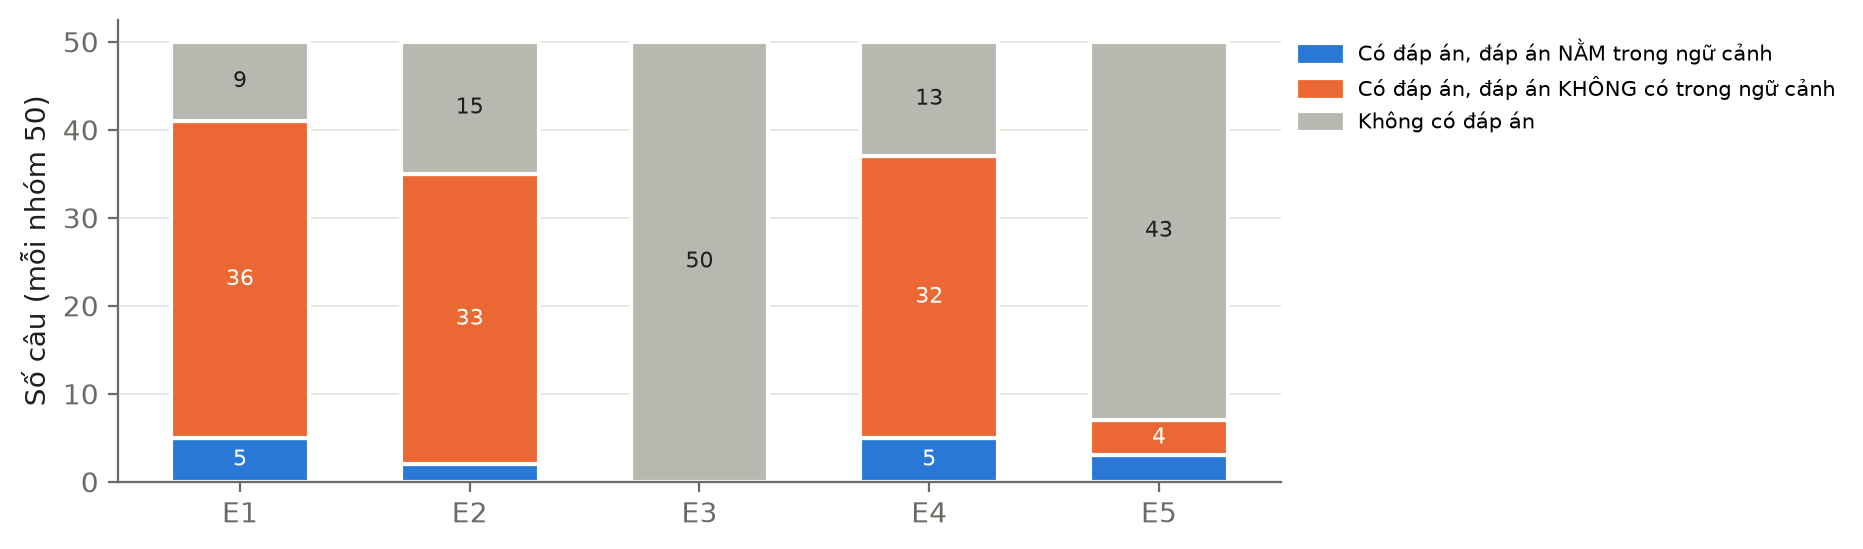
\includegraphics[width=0.88\textwidth]{figures/stress_audit.png}
\caption{Thành phần từng nhóm stress-test. Phần cam là câu có đáp án mà đáp án không nằm trong ngữ cảnh --- không mô hình trích xuất nào trả lời đúng được}
\label{fig:audit}
\end{figure}

Bốn phát hiện:

\begin{enumerate}
  \item \textbf{Đáp án không nằm trong ngữ cảnh.} Chỉ \AuditAnsInCtx{} trên \AuditAns{} câu có đáp
        án chứa đáp án vàng trong đoạn văn; chỉ \AuditOffsetOK{} câu có \code{answer\_start} đúng.
        Với các câu còn lại, điểm EM tối đa của \emph{mọi} mô hình trích xuất là 0.
  \item \textbf{Độ đa dạng rất thấp.} Cả 250 câu dùng chung \AuditCtx{} đoạn văn. Nhóm E5 có 50 câu
        nhưng chỉ \AuditEFiveDistinctQ{} câu hỏi khác nhau; nhóm E1 có \AuditEOneDistinctQ{}. Câu hỏi
        của E1 phần lớn là câu ``siêu ngôn ngữ'' dạng \emph{``Tại sao từ ghép `X' khó được tách từ
        chính xác trong ngữ cảnh này?''} với đáp án là chính X, nên 19 câu có đáp án nằm nguyên văn
        trong câu hỏi. Chúng đo khả năng chép lại cụm trong nháy đơn, không đo ranh giới từ ghép.
  \item \textbf{Mất cân bằng nhãn tạo điểm thoái hoá.} E3 có 100\% câu không có đáp án, E5 có 86\%.
        Hệ thống luôn từ chối đạt 100 điểm trên E3 và \AbstainStressEM{} điểm trên toàn bộ 250 câu.
  \item \textbf{Tệp gộp chứa bản ghi ngoài lược đồ.} Tệp \code{stress\_test\_combined.json} có
        \AuditCombined{} bản ghi: 250 câu SQuAD cộng \AuditFlat{} bản ghi ``phẳng'' không theo lược đồ
        SQuAD (24 mỗi nhóm) mà tài liệu dự án không nhắc tới. Đây là lời giải cho sự chênh lệch
        ``370 so với 250'' từng ghi nhận.
\end{enumerate}

\paragraph{Nguyên nhân gốc.} Truy ngược mã sinh dữ liệu (\code{legacy/stress\_test\_generator.py})
cho thấy hai lỗi ``sai âm thầm'' cụ thể: hàm \code{\_find\_answer\_start} trả về \textbf{0} khi không
tìm thấy đáp án trong ngữ cảnh thay vì báo lỗi; và hàm \code{\_wrap\_into\_squad} gán ngữ cảnh
\emph{theo vòng} cho các mẫu chưa có ngữ cảnh --- sau khi câu hỏi và đáp án đã được viết cho một
ngữ cảnh khác. Hai lỗi cộng lại tạo ra dữ liệu đúng định dạng, qua được mọi kiểm tra rò rỉ (báo cáo
rò rỉ đi kèm ghi \code{is\_clean: true}), nhưng sai về nội dung.

\paragraph{Hệ quả cho thiết kế.} Bộ stress-test được giữ lại \emph{như một đối tượng nghiên cứu},
không như một thước đo: các mô hình vẫn được chấm trên nó (Mục~\ref{sec:res-rq3}) để cho thấy điểm
số trên một bộ chẩn đoán lỗi trông như thế nào, nhưng không kết luận nào về mô hình dựa trên nó.
Vai trò chẩn đoán được chuyển sang các phép đo trên \emph{validation} --- \NValAns{} câu có đáp án do
người gán --- bắt đầu từ phép đo biên từ dưới đây. Đây đúng là điều kiện mà Bowman và Dahl
\cite{bowman2021fix} nêu: một bộ chẩn đoán chỉ có giá trị khi nhãn của nó đúng.

\subsection{Trần EM do biên từ}
\label{sec:alignment-res}

Phép đo ở Mục~\ref{sec:alignment} chạy trên toàn bộ \SegN{} câu có đáp án của validation, không cần
mô hình:

\begin{itemize}
  \item \textbf{\SegAligned{} câu (\SegAlignedPct\%)} có ít nhất một đáp án vàng khớp biên từ của
        \code{pyvi}. Chỉ \textbf{\SegMis{} câu (\SegMisPct\%)} có đáp án cắt ngang một từ (\SegStartCut{}
        câu cắt ở đầu, \SegEndCut{} câu cắt ở cuối).
  \item \textbf{Trần EM của một mô hình word-level hoàn hảo là \SegOracle\%}: kênh ``đơn vị đầu ra''
        của giả thuyết RQ1 chỉ lấy đi được tối đa \SegCeilingLoss{} điểm EM trên câu có đáp án.
  \item Trên chính \SegMis{} câu lệch biên, span nguyên-từ gần nhất vẫn đạt EM trong \SegOracleMis\%
        trường hợp, vì phần thừa chỉ là dấu câu mà bước chuẩn hoá xoá đi.
\end{itemize}

Đọc từng câu trong \SegMis{} câu lệch biên cùng kết quả tách từ xung quanh đáp án cho một bức tranh
khác hẳn giả thuyết (Bảng~\ref{tab:misaligned}): phần lớn \emph{không} phải là ranh giới từ ghép
khó của tiếng Việt, mà là \textbf{lỗi của bộ tách từ} và \textbf{lỗi gán nhãn}.

\begin{table}[htbp]
\centering
\caption{Phân loại \SegMis{} câu lệch biên từ trên validation (nguồn: \code{results/misaligned\_labels.json})}
\label{tab:misaligned}
\renewcommand{\arraystretch}{1.18}
\small
\begin{tabularx}{\textwidth}{@{}L r L@{}}
\toprule
\textbf{Nguyên nhân} & \textbf{Số câu} & \textbf{Ví dụ: tách từ quanh đáp án (\textbf{vàng})} \\
\midrule
\code{pyvi} dính dấu chấm vào token viết hoa (luật chữ viết tắt) & \MisPeriod & \code{như \textbf{CNN}.} $\to$ \code{CNN.}; \code{vua Ferdinand \textbf{VII}.} \\
\code{pyvi} nối nhầm âm tiết qua ranh giới từ & \MisMerge & \code{phim hoạt\_hình \textbf{Mỹ}\_Chú chuột}; \code{tại \textbf{Nam\_Phi}\_với} \\
Lỗi gán nhãn: đáp án vàng bị cắt giữa âm tiết & \MisAnnot & vàng ``\textbf{o thời gian} \dots'' (thiếu ``d''); ``\dots các nhà \textbf{thông thá}'' \\
Ranh giới từ ghép thật & \MisCompound & \code{bởi\_\textbf{vì}}; \code{vào\_\textbf{khoảng}} \\
\bottomrule
\end{tabularx}
\end{table}

\begin{keybox}
\textbf{Hệ quả cho RQ1.} Kênh ``PhoBERT không thể trả lời nửa từ'' giải thích được \emph{tối đa}
\SegCeilingLoss{} điểm EM trên câu có đáp án, và chỉ \MisCompound{} trong \SegMis{} câu lệch biên là ranh
giới từ ghép thật. Nếu PhoBERT kém XLM-R nhiều hơn mức đó, phần chênh còn lại phải đến từ kênh khác ---
biểu diễn, dữ liệu tiền huấn luyện, giới hạn 256 vị trí --- chứ không phải từ việc đáp án cắt ngang từ
ghép. Ngược lại, các lỗi của \code{pyvi} ở bảng trên (nối nhầm âm tiết, dính dấu câu) là những lỗi
\emph{cũng xảy ra bên trong ngữ cảnh}, và chúng đi vào biểu diễn đầu vào của PhoBERT ở mọi câu, không
chỉ ở câu lệch biên.
\end{keybox}

\subsection{Kết quả tổng}
\label{sec:res-main}

\begin{table}[htbp]
\centering
\caption{Kết quả trên toàn bộ validation (\NVal{} câu; nguồn: \code{results/eval\_*\_validation.json})}
\label{tab:main}
\renewcommand{\arraystretch}{1.18}
\footnotesize
\setlength{\tabcolsep}{4pt}
\begin{tabularx}{\textwidth}{@{}L r r r r r r r@{}}
\toprule
& \multicolumn{2}{c}{\textbf{Toàn bộ}} & \multicolumn{2}{c}{\textbf{Có đáp án}} & \textbf{Không đáp án} & \textbf{Tỉ lệ} & \textbf{Độ trễ} \\
\cmidrule(lr){2-3}\cmidrule(lr){4-5}\cmidrule(lr){6-6}
\textbf{Hệ thống} & \textbf{EM} & \textbf{F1} & \textbf{EM} & \textbf{F1} & \textbf{EM} & \textbf{từ chối} & \textbf{ms/câu} \\
\midrule
\tabinput{generated/tab_main.tex}
\bottomrule
\end{tabularx}
\end{table}

\begin{figure}[htbp]
\centering
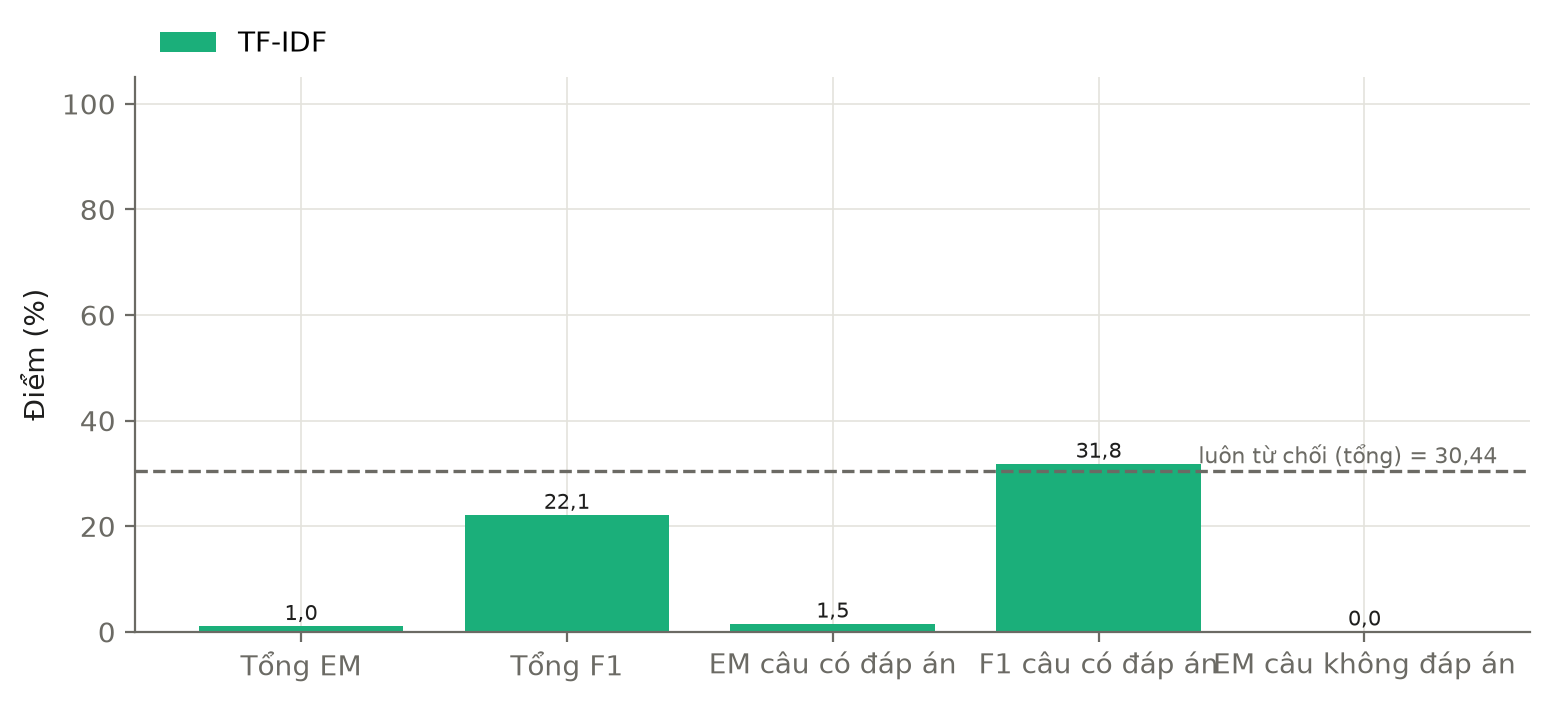
\includegraphics[width=\textwidth]{figures/main_results.png}
\caption{Kết quả chính. Đường đứt: điểm tổng của hệ thống luôn từ chối}
\label{fig:main}
\end{figure}

%RESULTS-MAIN-PROSE

\subsection{RQ1 --- Mô hình word-level có nhạy với ranh giới từ hơn?}
\label{sec:res-rq1}

\begin{table}[htbp]
\centering
\caption{EM/F1 theo tương thích biên từ của đáp án vàng (câu có đáp án)}
\label{tab:alignment}
\renewcommand{\arraystretch}{1.15}
\small
\begin{tabular}{@{}l r r r r@{}}
\toprule
& \multicolumn{2}{c}{\textbf{Khớp biên (\SegAligned{} câu)}} & \multicolumn{2}{c}{\textbf{Lệch biên (\SegMis{} câu)}} \\
\cmidrule(lr){2-3}\cmidrule(lr){4-5}
\textbf{Hệ thống} & \textbf{EM} & \textbf{F1} & \textbf{EM} & \textbf{F1} \\
\midrule
\tabinput{generated/tab_alignment.tex}
\bottomrule
\end{tabular}
\end{table}

\begin{table}[htbp]
\centering
\caption{Phân loại lỗi trên toàn bộ validation (số câu; định nghĩa ở Bảng~\ref{tab:taxonomy-def})}
\label{tab:taxonomy}
\renewcommand{\arraystretch}{1.15}
\footnotesize
\setlength{\tabcolsep}{4pt}
\begin{tabularx}{\textwidth}{@{}L r r r r r r r@{}}
\toprule
\textbf{Hệ thống} & \textbf{Tổng lỗi} & \textbf{Từ chối sai} & \textbf{Trả lời sai} & \textbf{Biên thừa} & \textbf{Biên thiếu} & \textbf{Biên lệch} & \textbf{Sai vị trí} \\
\midrule
\tabinput{generated/tab_taxonomy.tex}
\bottomrule
\end{tabularx}
\end{table}

\begin{figure}[htbp]
\centering
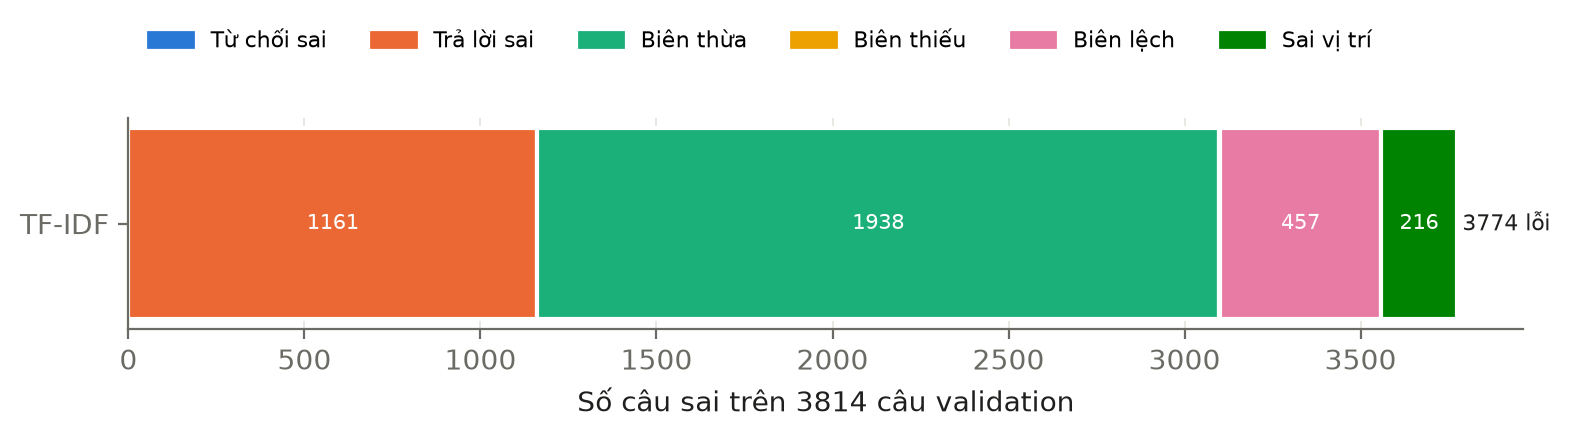
\includegraphics[width=\textwidth]{figures/error_taxonomy.png}
\caption{Cơ cấu lỗi của từng hệ thống}
\label{fig:taxonomy}
\end{figure}

\begin{table}[htbp]
\centering
\caption{So sánh cặp PhoBERT (A) và XLM-R (B) theo EM từng câu. Chênh lệch = EM(A) $-$ EM(B), điểm \%}
\label{tab:paired}
\renewcommand{\arraystretch}{1.15}
\footnotesize
\setlength{\tabcolsep}{4pt}
\begin{tabularx}{\textwidth}{@{}L r r r r r r l r@{}}
\toprule
\textbf{Nhóm câu} & $n$ & \textbf{Cả hai đúng} & \textbf{Chỉ A} & \textbf{Chỉ B} & \textbf{Cả hai sai} & \textbf{Chênh lệch} & \textbf{CI 95\%} & \textbf{$p$ McNemar} \\
\midrule
\tabinput{generated/tab_paired.tex}
\bottomrule
\end{tabularx}
\end{table}

%RESULTS-RQ1-PROSE

\subsection{RQ2 --- Độ dài ngữ cảnh và độ dài đáp án}
\label{sec:res-rq2}

\begin{table}[htbp]
\centering
\caption{EM / F1 theo độ dài đoạn văn (âm tiết). $^\dagger$: nhóm dưới 30 câu}
\label{tab:ctxlen}
\renewcommand{\arraystretch}{1.15}
\footnotesize
\begin{tabular}{@{}l r r r r r@{}}
\toprule
\textbf{Độ dài} & $n$ & \textbf{Luôn từ chối} & \textbf{TF-IDF} & \textbf{XLM-R} & \textbf{PhoBERT} \\
\midrule
\tabinput{generated/tab_context_length.tex}
\bottomrule
\end{tabular}
\end{table}

\begin{table}[htbp]
\centering
\caption{EM / F1 theo độ dài đáp án vàng (âm tiết; câu có đáp án)}
\label{tab:anslen}
\renewcommand{\arraystretch}{1.15}
\footnotesize
\begin{tabular}{@{}l r r r r@{}}
\toprule
\textbf{Hệ thống} & \textbf{1--2 (\NLenOne)} & \textbf{3--5 (\NLenThree)} & \textbf{6--10 (\NLenSix)} & \textbf{11+ (\NLenEleven)} \\
\midrule
\tabinput{generated/tab_answer_length.tex}
\bottomrule
\end{tabular}
\end{table}

\begin{figure}[htbp]
\centering
\begin{subfigure}{0.49\textwidth}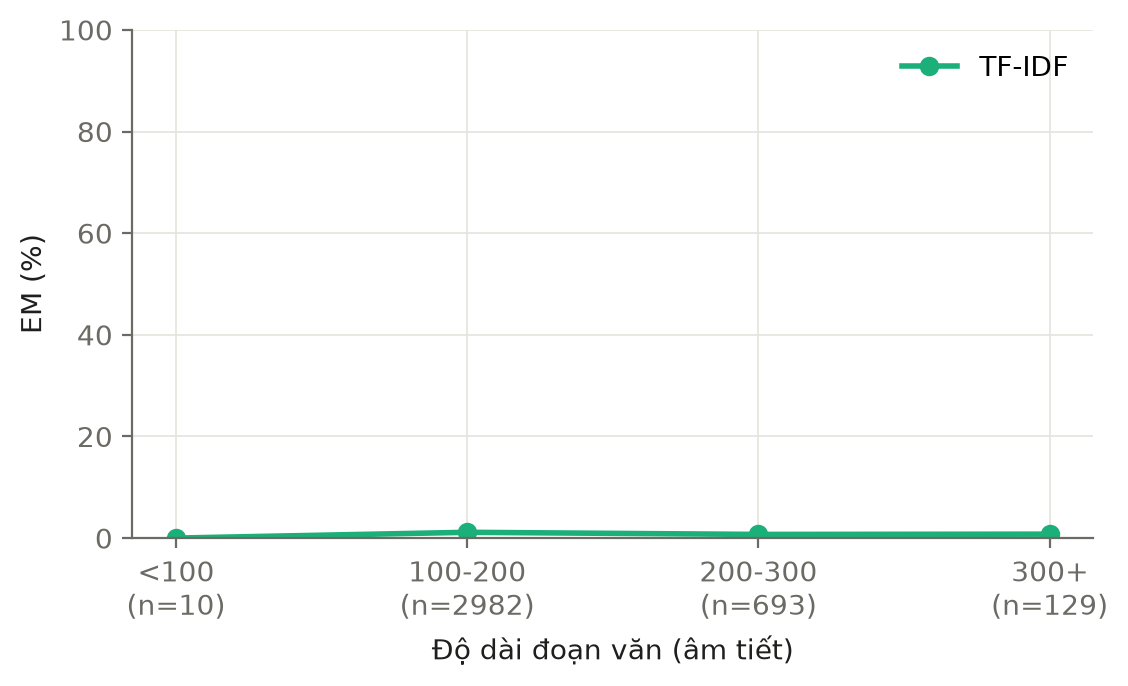
\includegraphics[width=\textwidth]{figures/by_context_length.png}\caption{Theo độ dài đoạn văn}\end{subfigure}
\hfill
\begin{subfigure}{0.49\textwidth}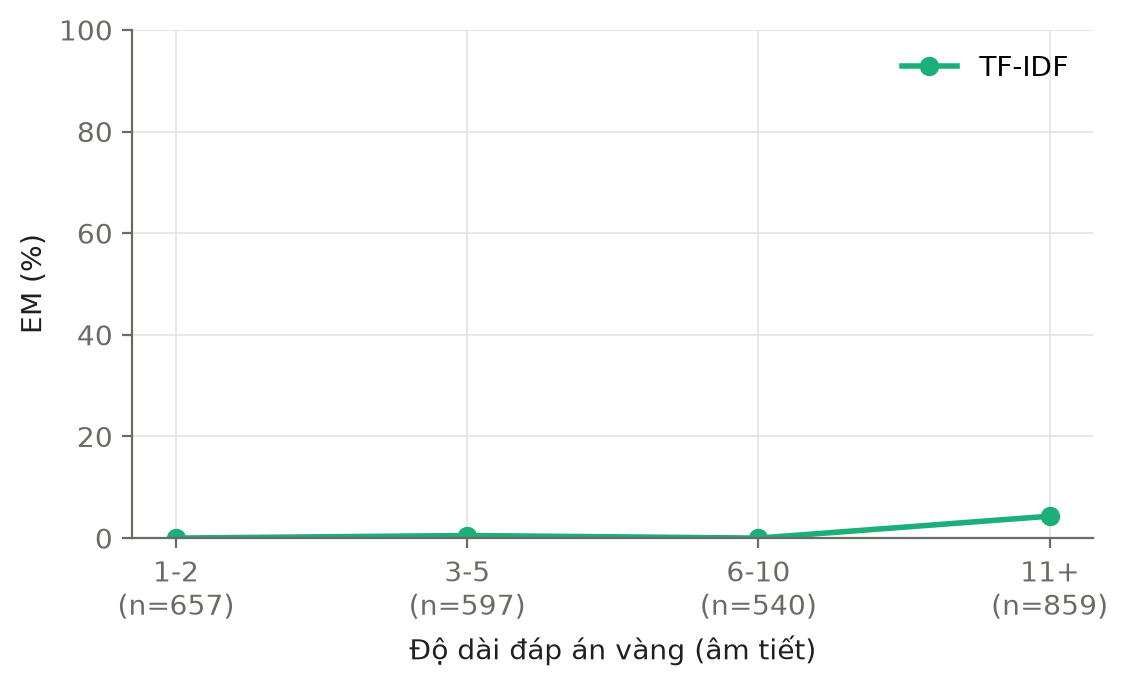
\includegraphics[width=\textwidth]{figures/by_answer_length.png}\caption{Theo độ dài đáp án}\end{subfigure}
\caption{EM theo độ dài}
\label{fig:lengths}
\end{figure}

%RESULTS-RQ2-PROSE

\subsection{RQ3 --- Nhận ra câu không có đáp án, hay thiên lệch về từ chối?}
\label{sec:res-rq3}

\begin{table}[htbp]
\centering
\caption{Hành vi từ chối như một bộ phân loại ``không có đáp án'' (validation)}
\label{tab:abstention}
\renewcommand{\arraystretch}{1.15}
\small
\begin{tabular}{@{}l r r r@{}}
\toprule
\textbf{Hệ thống} & \textbf{Tỉ lệ từ chối (\%)} & \textbf{Precision (\%)} & \textbf{Recall (\%)} \\
\midrule
Luôn từ chối & \AbstainAbsRate & \AbstainAbsPrec & \AbstainAbsRec \\
XLM-R-base & \XlmrAbsRate & \XlmrAbsPrec & \XlmrAbsRec \\
PhoBERT-base-v2 & \PhobertAbsRate & \PhobertAbsPrec & \PhobertAbsRec \\
\bottomrule
\end{tabular}
\par\vspace{2pt}{\footnotesize Tỉ lệ câu không có đáp án thật: \PctValImp\%.}
\end{table}

\begin{table}[htbp]
\centering
\caption{EM trên bộ stress-test theo nhóm: \emph{toàn bộ} / \emph{chỉ câu hợp lệ}. Chỉ để minh hoạ --- xem Mục~\ref{sec:audit}}
\label{tab:stress}
\renewcommand{\arraystretch}{1.15}
\footnotesize
\setlength{\tabcolsep}{4pt}
\begin{tabular}{@{}l r r r r r r@{}}
\toprule
\textbf{Hệ thống} & \textbf{E1} & \textbf{E2} & \textbf{E3} & \textbf{E4} & \textbf{E5} & \textbf{Tổng} \\
\midrule
\tabinput{generated/tab_stress.tex}
\bottomrule
\end{tabular}
\par\vspace{2pt}{\footnotesize Số câu hợp lệ mỗi nhóm: E1 \AuditEOneValid, E2 \AuditETwoValid, E3 \AuditEThreeValid, E4 \AuditEFourValid, E5 \AuditEFiveValid.}
\end{table}

%RESULTS-RQ3-PROSE

\subsection{RQ4 --- Transformer có vượt baseline ở mọi nhóm?}
\label{sec:res-rq4}

%RESULTS-RQ4-PROSE

\subsection{Phân tích định tính}
\label{sec:qualitative}

%RESULTS-QUAL-PROSE

\subsection{Quá trình huấn luyện và chi phí}
\label{sec:curves}

\begin{table}[htbp]
\centering
\caption{Đường cong huấn luyện. EM/F1 đo trên dev (500 câu ngẫu nhiên tách từ train). $\star$: epoch được chọn}
\label{tab:curves}
\renewcommand{\arraystretch}{1.15}
\small
\begin{tabular}{@{}l c r r r r@{}}
\toprule
\textbf{Mô hình} & \textbf{Epoch} & \textbf{Loss} & \textbf{EM dev} & \textbf{F1 dev} & \textbf{Phút} \\
\midrule
\tabinput{generated/tab_curves.tex}
\bottomrule
\end{tabular}
\end{table}

\begin{figure}[htbp]
\centering
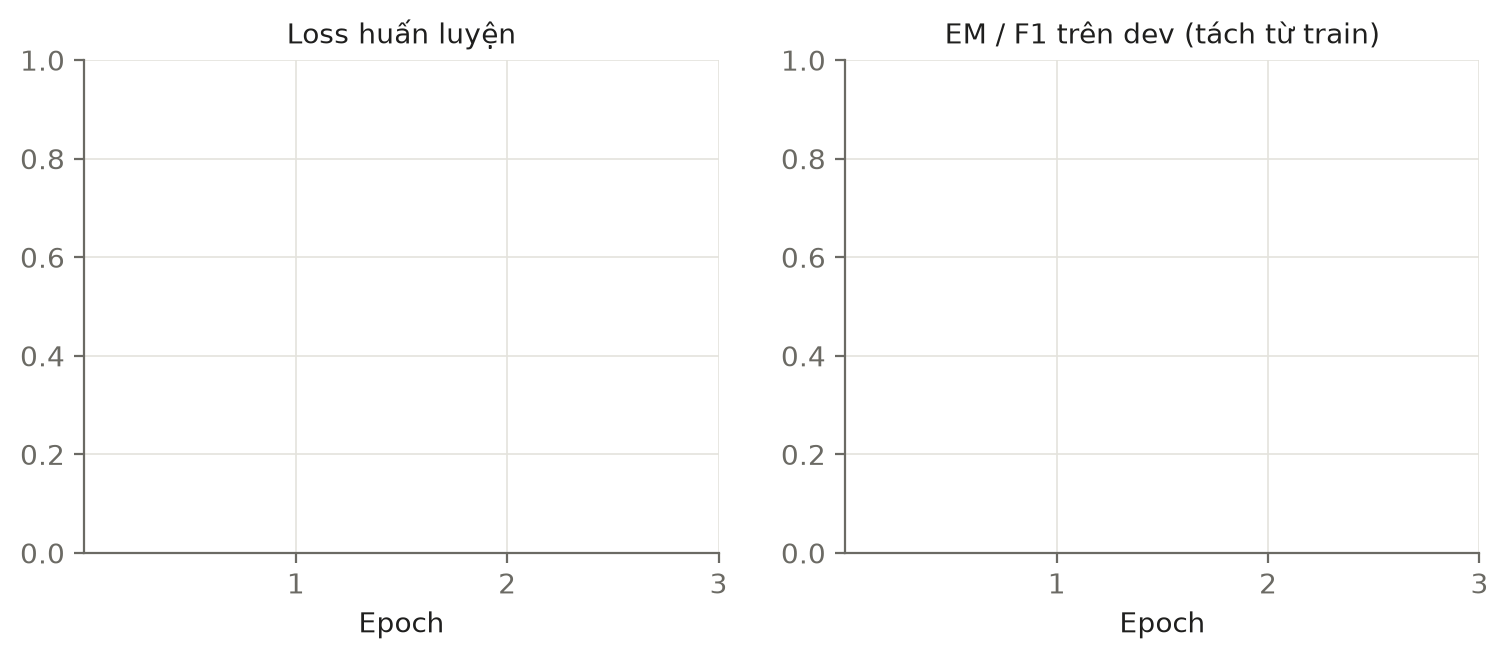
\includegraphics[width=\textwidth]{figures/training_curves.png}
\caption{Loss huấn luyện và EM/F1 trên dev theo epoch}
\label{fig:curves}
\end{figure}

%RESULTS-CURVES-PROSE

% ============================================================================
\section{Kết luận}
\label{sec:conclusion}
% ============================================================================

\subsection{Kết luận}

Đồ án khảo sát hai mô hình Transformer tiền huấn luyện cho đọc hiểu trích xuất tiếng Việt --- PhoBERT
(đơn ngữ, word-level) và XLM-R (đa ngữ, subword) --- được fine-tune trong cùng điều kiện trên
UIT-ViQuAD~2.0 và chấm một lần trên toàn bộ \NVal{} câu validation. Bốn câu hỏi nghiên cứu được trả lời
như sau.

\begin{enumerate}
  \item \textbf{RQ1 --- ranh giới từ.} Giả thuyết ghi trước (PhoBERT yếu hơn vì lỗi tách từ) \emph{sai}
        ở dạng tổng quát: PhoBERT hơn XLM-R \PairAnsDiff{} điểm EM trên câu có đáp án, và tỉ lệ lỗi biên
        khi đã trả lời của hai mô hình như nhau (\PhobertBoundaryRate\% và \XlmrBoundaryRate\%). Cơ chế
        ``không trả lời được nửa từ'' có thật, nhìn thấy được qua dấu hiệu F1 cao/EM thấp, nhưng chỉ tác
        động lên \SegMisPct\% câu hỏi và bị chặn trên ở \SegCeilingLoss{} điểm EM; phần lớn các câu đó là lỗi
        của bộ tách từ \code{pyvi}, không phải ranh giới từ ghép thật.
  \item \textbf{RQ2 --- độ dài.} Không có suy giảm theo độ dài ngữ cảnh ở cả hai họ mô hình; độ dài đáp án
        làm giảm EM (không giảm F1) như nhau ở cả hai.
  \item \textbf{RQ3 --- câu không có đáp án.} Không mô hình nào thật sự nhận ra câu không có đáp án. XLM-R từ
        chối đúng tần suất nhưng sai đối tượng (precision \XlmrAbsPrec\%); PhoBERT gần như không từ chối
        (\PhobertAbsRate\%), vì loss trên lớp ``không có đáp án'' của nó tăng khoảng 7 lần sau epoch 1 trong
        khi loss trên vị trí đáp án vẫn giảm --- lặp lại ở hai tốc độ học. Cả hai thường trả về đúng cụm
        gây nhiễu mà người gán nhãn đặt vào câu hỏi.
  \item \textbf{RQ4 --- baseline.} Transformer vượt TF-IDF ở mọi nhóm; TF-IDF thậm chí không vượt được hệ
        thống luôn từ chối về EM tổng.
\end{enumerate}

\paragraph{Điều rút ra.} Điểm tổng của PhoBERT và XLM-R không khác nhau có ý nghĩa thống kê, nhưng hai mô
hình có hai hồ sơ kỹ năng ngược nhau: một mô hình đọc giỏi mà không biết từ chối, một mô hình biết từ chối
nhưng từ chối nhầm chỗ. Chọn mô hình dựa trên điểm tổng sẽ bỏ qua điều quan trọng nhất cho triển khai. Với
câu hỏi ban đầu của môn học --- \emph{đặc điểm dữ liệu quyết định phương pháp} --- câu trả lời của đồ án là:
trên UIT-ViQuAD~2.0, đặc điểm quyết định không phải là tách từ mà là \emph{một phần ba câu hỏi không có đáp
án}; và việc một mô hình xử lý phần đó ra sao phải được đo riêng.

\paragraph{Về phương pháp.} Hai trong ba công cụ chẩn đoán có giá trị nhất của đồ án không cần chạy mô hình
nào: phép đo biên từ cho biết trước giới hạn trên của hiệu ứng mà giả thuyết RQ1 dự đoán, và phép kiểm định
bộ stress-test cho thấy bộ dữ liệu chẩn đoán do chính nhóm xây \emph{không đo được thứ nó tuyên bố đo}. Nếu
không kiểm định, bảng kết quả trên bộ đó sẽ xếp ``không làm gì'' đứng đầu mà không ai nhận ra vì sao.

\subsection{Giới hạn}
\label{sec:limitations}

Các giới hạn dưới đây quyết định phạm vi mà mọi kết luận ở trên có giá trị.

\begin{enumerate}
  \item \textbf{Một seed huấn luyện cho mỗi mô hình.} Kiểm định McNemar và bootstrap đo độ bất định do
        \emph{chọn câu hỏi}, không đo độ bất định do \emph{seed}. Với mô hình cỡ base trên SQuAD, chênh
        lệch giữa các seed có thể lên tới một vài điểm EM; một chênh lệch nhỏ hơn cỡ đó không nên được
        hiểu là khác biệt giữa hai \emph{kiến trúc}.
  \item \textbf{Không tìm kiếm siêu tham số.} Cả hai mô hình dùng cùng một cấu hình phổ biến; mỗi mô
        hình có thể đạt điểm cao hơn ở cấu hình riêng của nó. So sánh ở đây là ``cùng điều kiện'', không
        phải ``mỗi bên ở trạng thái tốt nhất''.
  \item \textbf{Bộ tách từ khác với lúc tiền huấn luyện.} PhoBERT được tiền huấn luyện trên văn bản tách
        bởi RDRSegmenter; đồ án dùng \code{pyvi} để không phụ thuộc Java. Lệch phân phối này có thể làm
        PhoBERT kém hơn khả năng thật của nó, và Mục~\ref{sec:alignment-res} cho thấy \code{pyvi} có những
        lỗi hệ thống (dính dấu chấm, nối nhầm âm tiết).
  \item \textbf{Validation đóng vai tập test.} Test chính thức ẩn nhãn nên không chấm được. Validation
        không được dùng cho bất kỳ quyết định nào trước khi chấm (Mục~\ref{sec:protocol}), nhưng kết quả
        không so sánh trực tiếp được với các con số công bố trên test của cuộc thi VLSP.
  \item \textbf{Giới hạn vị trí khác nhau là một phần của so sánh.} PhoBERT dùng 256 token, XLM-R 384
        token. Đây là ràng buộc kiến trúc chứ không phải lựa chọn, nhưng nó có nghĩa là ``PhoBERT vs XLM-R''
        không cô lập riêng biến tokenization.
  \item \textbf{Bộ stress-test không dùng được làm thước đo} (Mục~\ref{sec:audit}). Các nhóm hiện tượng
        E2--E5 vì vậy không có bằng chứng định lượng đáng tin cậy trong đồ án này; phân tích theo độ dài và
        theo loại lỗi trên validation chỉ thay thế được một phần.
  \item \textbf{Phân loại thủ công 33 câu lệch biên} do một người thực hiện, chưa đo độ đồng thuận giữa
        các người gán. Phân loại lỗi tự động (Mục~\ref{sec:taxonomy}) dựa trên quan hệ tập hợp token nên
        tái lập được, nhưng không phân biệt được lỗi ``hiểu sai câu hỏi'' với ``chọn nhầm thực thể cùng loại''.
  \item \textbf{Miền dữ liệu.} Toàn bộ dữ liệu là Wikipedia; kết luận không tự động mở rộng sang văn bản
        mạng xã hội, nơi lỗi tách từ được dự đoán còn nặng hơn.
\end{enumerate}

\subsection{Hướng phát triển}
\label{sec:future}

\begin{enumerate}
  \item \textbf{Hiệu chỉnh ngưỡng từ chối trên dev.} Ngưỡng $\tau$ trong công thức~(\ref{eq:null}) được cố định
        bằng 0. Chọn $\tau$ riêng cho từng mô hình trên tập dev (không phải validation) là cách rẻ nhất để
        thử khôi phục khả năng từ chối của PhoBERT; kết quả cần được chấm lại trên validation.
  \item \textbf{Tìm nguyên nhân gốc của việc PhoBERT bỏ lớp ``không có đáp án''}: nhiều seed, ghi lại chuẩn
        gradient theo loại nhãn, thử trọng số lớp, thử độ dài 256 cho XLM-R để tách biến ``độ dài cửa sổ''
        khỏi biến ``mô hình''.
  \item \textbf{Bộ tách từ.} Chạy lại PhoBERT với RDRSegmenter (VnCoreNLP) --- bộ tách từ dùng lúc tiền
        huấn luyện --- để đo phần hiệu năng bị mất do lệch bộ tách từ; và sửa luật dính dấu chấm của
        \code{pyvi}, nguyên nhân của \MisPeriod{} trong \SegMis{} câu lệch biên.
  \item \textbf{Xây lại bộ stress-test} theo quy trình có kiểm định tự động từ đầu: đáp án phải nằm trong
        ngữ cảnh (báo lỗi thay vì trả về 0), mỗi nhóm có đủ câu có đáp án làm đối chứng, và câu hỏi do người
        viết thay vì sinh từ khuôn mẫu; đo độ đồng thuận giữa người gán.
  \item \textbf{Nhiều seed} cho mọi mô hình để tách độ bất định do huấn luyện khỏi độ bất định do chọn câu
        hỏi.
\end{enumerate}

% ============================================================================
\phantomsection
\addcontentsline{toc}{section}{Tài liệu tham khảo}
{\setstretch{1.0}\footnotesize
\begin{thebibliography}{99}\setlength{\itemsep}{1pt}\setlength{\parskip}{0pt}

\bibitem{nguyen2020viquad}
K.~V. Nguyen, D.-V. Nguyen, A.~G.-T. Nguyen, and N.~L.-T. Nguyen.
\newblock A Vietnamese dataset for evaluating machine reading comprehension.
\newblock In \emph{Proceedings of the 28th International Conference on Computational Linguistics (COLING)}, pages 2595--2605, 2020.

\bibitem{nguyen2022vlsp}
K.~V. Nguyen, S.~Q. Tran, L.~T. Nguyen, T.~V. Huynh, S.~T. Luu, and N.~L.-T. Nguyen.
\newblock VLSP 2021 -- ViMRC challenge: Vietnamese machine reading comprehension.
\newblock \emph{arXiv preprint arXiv:2203.11400}, 2022.

\bibitem{rajpurkar2016squad}
P.~Rajpurkar, J.~Zhang, K.~Lopyrev, and P.~Liang.
\newblock SQuAD: 100,000+ questions for machine comprehension of text.
\newblock In \emph{Proceedings of the 2016 Conference on Empirical Methods in Natural Language Processing (EMNLP)}, pages 2383--2392, 2016.

\bibitem{rajpurkar2018know}
P.~Rajpurkar, R.~Jia, and P.~Liang.
\newblock Know what you don't know: Unanswerable questions for SQuAD.
\newblock In \emph{Proceedings of the 56th Annual Meeting of the Association for Computational Linguistics (ACL)}, pages 784--789, 2018.

\bibitem{vaswani2017attention}
A.~Vaswani, N.~Shazeer, N.~Parmar, J.~Uszkoreit, L.~Jones, A.~N. Gomez, Ł.~Kaiser, and I.~Polosukhin.
\newblock Attention is all you need.
\newblock In \emph{Advances in Neural Information Processing Systems (NeurIPS)}, 2017.

\bibitem{devlin2019bert}
J.~Devlin, M.-W. Chang, K.~Lee, and K.~Toutanova.
\newblock BERT: Pre-training of deep bidirectional transformers for language understanding.
\newblock In \emph{Proceedings of NAACL-HLT}, pages 4171--4186, 2019.

\bibitem{conneau2020xlmr}
A.~Conneau, K.~Khandelwal, N.~Goyal, V.~Chaudhary, G.~Wenzek, F.~Guzmán, E.~Grave, M.~Ott, L.~Zettlemoyer, and V.~Stoyanov.
\newblock Unsupervised cross-lingual representation learning at scale.
\newblock In \emph{Proceedings of the 58th Annual Meeting of the Association for Computational Linguistics (ACL)}, pages 8440--8451, 2020.

\bibitem{nguyen2020phobert}
D.~Q. Nguyen and A.~T. Nguyen.
\newblock PhoBERT: Pre-trained language models for Vietnamese.
\newblock In \emph{Findings of the Association for Computational Linguistics: EMNLP 2020}, pages 1037--1042, 2020.

\bibitem{kudo2018sentencepiece}
T.~Kudo and J.~Richardson.
\newblock SentencePiece: A simple and language independent subword tokenizer and detokenizer for neural text processing.
\newblock In \emph{Proceedings of EMNLP 2018: System Demonstrations}, pages 66--71, 2018.

\bibitem{loshchilov2019adamw}
I.~Loshchilov and F.~Hutter.
\newblock Decoupled weight decay regularization.
\newblock In \emph{International Conference on Learning Representations (ICLR)}, 2019.

\bibitem{pedregosa2011sklearn}
F.~Pedregosa, G.~Varoquaux, A.~Gramfort, V.~Michel, B.~Thirion, et~al.
\newblock Scikit-learn: Machine learning in Python.
\newblock \emph{Journal of Machine Learning Research}, 12:2825--2830, 2011.

\bibitem{paszke2019pytorch}
A.~Paszke, S.~Gross, F.~Massa, A.~Lerer, J.~Bradbury, et~al.
\newblock PyTorch: An imperative style, high-performance deep learning library.
\newblock In \emph{Advances in Neural Information Processing Systems (NeurIPS)}, 2019.

\bibitem{wolf2020transformers}
T.~Wolf, L.~Debut, V.~Sanh, J.~Chaumond, C.~Delangue, et~al.
\newblock Transformers: State-of-the-art natural language processing.
\newblock In \emph{Proceedings of EMNLP 2020: System Demonstrations}, pages 38--45, 2020.

\bibitem{liu2019roberta}
Y.~Liu, M.~Ott, N.~Goyal, J.~Du, M.~Joshi, D.~Chen, O.~Levy, M.~Lewis, L.~Zettlemoyer, and V.~Stoyanov.
\newblock RoBERTa: A robustly optimized BERT pretraining approach.
\newblock \emph{arXiv preprint arXiv:1907.11692}, 2019.

\bibitem{sennrich2016bpe}
R.~Sennrich, B.~Haddow, and A.~Birch.
\newblock Neural machine translation of rare words with subword units.
\newblock In \emph{Proceedings of the 54th Annual Meeting of the Association for Computational Linguistics (ACL)}, pages 1715--1725, 2016.

\bibitem{vu2018vncorenlp}
T.~Vu, D.~Q. Nguyen, D.~Q. Nguyen, M.~Dras, and M.~Johnson.
\newblock VnCoreNLP: A Vietnamese natural language processing toolkit.
\newblock In \emph{Proceedings of NAACL-HLT 2018: Demonstrations}, pages 56--60, 2018.

\bibitem{pyvi}
V.~T. Tran.
\newblock \code{pyvi}: Python Vietnamese core NLP toolkit.
\newblock \url{https://github.com/trungtv/pyvi}.

\bibitem{jia2017adversarial}
R.~Jia and P.~Liang.
\newblock Adversarial examples for evaluating reading comprehension systems.
\newblock In \emph{Proceedings of the 2017 Conference on Empirical Methods in Natural Language Processing (EMNLP)}, pages 2021--2031, 2017.

\bibitem{naik2018stress}
A.~Naik, A.~Ravichander, N.~Sadeh, C.~Rose, and G.~Neubig.
\newblock Stress test evaluation for natural language inference.
\newblock In \emph{Proceedings of the 27th International Conference on Computational Linguistics (COLING)}, pages 2340--2353, 2018.

\bibitem{gardner2020contrast}
M.~Gardner, Y.~Artzi, V.~Basmov, J.~Berant, B.~Bogin, et~al.
\newblock Evaluating models' local decision boundaries via contrast sets.
\newblock In \emph{Findings of the Association for Computational Linguistics: EMNLP 2020}, pages 1307--1323, 2020.

\bibitem{ribeiro2020checklist}
M.~T. Ribeiro, T.~Wu, C.~Guestrin, and S.~Singh.
\newblock Beyond accuracy: Behavioral testing of NLP models with CheckList.
\newblock In \emph{Proceedings of the 58th Annual Meeting of the Association for Computational Linguistics (ACL)}, pages 4902--4912, 2020.

\bibitem{bowman2021fix}
S.~R. Bowman and G.~E. Dahl.
\newblock What will it take to fix benchmarking in natural language understanding?
\newblock In \emph{Proceedings of NAACL-HLT 2021}, pages 4843--4855, 2021.

\bibitem{dror2018hitchhiker}
R.~Dror, G.~Baumer, S.~Shlomov, and R.~Reichart.
\newblock The hitchhiker's guide to testing statistical significance in natural language processing.
\newblock In \emph{Proceedings of the 56th Annual Meeting of the Association for Computational Linguistics (ACL)}, pages 1383--1392, 2018.

\bibitem{mcnemar1947}
Q.~McNemar.
\newblock Note on the sampling error of the difference between correlated proportions or percentages.
\newblock \emph{Psychometrika}, 12(2):153--157, 1947.

\bibitem{efron1993bootstrap}
B.~Efron and R.~J. Tibshirani.
\newblock \emph{An Introduction to the Bootstrap}.
\newblock Chapman \& Hall, 1993.

\end{thebibliography}
}

% ============================================================================
%  PHỤ LỤC
% ============================================================================
\clearpage
\appendix
\renewcommand{\thesection}{\Alph{section}}
\titleformat{\section}{\normalfont\Large\bfseries}{Phụ lục \thesection.}{0.6em}{}

\section{Hướng dẫn tái lập}
\label{app:repro}

Toàn bộ kết quả tái lập được bằng các lệnh sau trên một máy có Python 3.12 (GPU không bắt buộc
cho phần đánh giá baseline và phân tích; bắt buộc trên thực tế cho fine-tune).

\begin{lstlisting}[language=bash,escapeinside={(*}{*)}]
# 1. (*\lstcmt{Môi trường và dữ liệu}*)
uv venv .venv --python 3.12
uv pip install --python .venv/bin/python -r requirements.txt
python scripts/fetch_data.py                   # UIT-ViQuAD 2.0 -> data/raw/

# 2. (*\lstcmt{Kiểm thử (không cần}*) GPU)
python -m pytest -m "not slow"

# 3. (*\lstcmt{Phân tích không cần mô hình}*)
python scripts/analyze_segmentation.py         # (*\lstcmt{biên từ + trần}*) EM
python scripts/build_stress_v2.py              # (*\lstcmt{dựng + kiểm định}*) stress-test v2

# 4. Fine-tune (dev (*\lstcmt{tách từ train; validation không được nhìn thấy)}*)
python scripts/finetune.py --model FacebookAI/xlm-roberta-base --out models/xlmr \
    --epochs 3 --max-length 384 --doc-stride 128 --max-answer-len 64
python scripts/finetune.py --model vinai/phobert-base-v2 --out models/phobert \
    --word-segmented --epochs 3 --max-length 256 --doc-stride 96 --max-answer-len 64
bash scripts/queue_night1.sh && bash scripts/queue_night2.sh   # seed 13, lr 1e-5, 256/96

# 5. (*\lstcmt{Chấm (mỗi hệ thống một lần, toàn bộ validation), chọn tau trên dev, chẩn đoán}*)
python scripts/run_eval.py --models abstain baseline xlmr phobert
python scripts/run_eval.py --models abstain baseline xlmr xlmr_seed13 phobert \
    phobert_seed13 xlmr_256 --dataset stress2
bash scripts/queue_score_windows.sh
python scripts/calibrate_thresholds.py --runs xlmr xlmr_seed13 xlmr_256 phobert \
    phobert_seed13 phobert_lr2e5 phobert_stable
python scripts/diagnose.py

# 5b. Stress-test v2 (*\lstcmt{ở tau chọn trên dev (không chọn gì trên}*) stress2)
for m in xlmr xlmr_seed13 phobert phobert_seed13 xlmr_256; do
  python scripts/score_windows.py --checkpoint models/$m --name $m --split stress2
done
python scripts/score_stress2_tuned.py --check-tau0 \
    --runs xlmr xlmr_seed13 phobert phobert_seed13 xlmr_256

# 6. (*\lstcmt{Báo cáo: số liệu và hình sinh từ results/, rồi biên dịch}*)
python scripts/make_report_numbers.py && python scripts/make_figures.py
cd report && latexmk -xelatex main.tex
\end{lstlisting}

\section{Kiểm định khung mã ban đầu}
\label{app:legacy}

Trước khi chạy bất kỳ thí nghiệm nào, nhóm rà soát khung mã ban đầu của đồ án (nay ở
\code{legacy/}). Rà soát cho thấy khung mã \emph{chưa từng được chạy} (không có tệp kết quả
hay checkpoint nào) nhưng tài liệu đi kèm đã trình bày số liệu. Các phát hiện được liệt kê để
người đọc biết vì sao khung mã này không được dùng, và vì sao báo cáo có quy tắc ``không con số
nào không có tệp kết quả''.

\begin{table}[H]
\centering
\caption{Các lỗi phát hiện trong khung mã ban đầu}
\label{tab:legacy}
\renewcommand{\arraystretch}{1.18}
\small
\begin{tabularx}{\textwidth}{@{}L L L@{}}
\toprule
\textbf{Lỗi} & \textbf{Hệ quả nếu chạy} & \textbf{Xử lý} \\
\midrule
Ba bộ số liệu kết quả khác nhau (README, slide, hằng \code{EXPECTED\_RESULTS}), không bộ nào có tệp nguồn & Báo cáo số không đo & Xoá toàn bộ; mọi số sinh từ \code{results/} \\
\code{compute\_metrics} so sánh chuỗi \code{"span\_\{s\}\_\{e\}"} thay vì văn bản đáp án; F1 được ``ước lượng'' bằng \code{EM $\times$ 0,95} & EM/F1 vô nghĩa & Giải mã span thật từ offset (Mục~\ref{sec:segtok}) \\
Giải mã PhoBERT giữ dấu ``\_'' của bước tách từ & Đáp án đúng bị chấm EM~0 & Cắt đáp án từ văn bản gốc; kiểm thử hồi quy \\
Ghi đè \code{max\_position\_embeddings} của PhoBERT & Hỏng embedding vị trí khi nạp & Bỏ; \code{max\_length} = 256 \\
\code{include\_stress\_test=True} mặc định: 60\% bộ stress-test bị trộn vào tập \emph{huấn luyện} & Rò rỉ: chấm trên dữ liệu đã học & Stress-test chỉ dùng để đánh giá \\
Bộ sinh stress-test: \code{\_find\_answer\_start} trả về 0 khi không tìm thấy đáp án; \code{\_wrap\_into\_squad} gán lại ngữ cảnh theo vòng cho mẫu không có ngữ cảnh & Phần lớn câu có đáp án không nằm trong ngữ cảnh: bộ cũ không đo được thứ nó tuyên bố đo & Dựng lại bộ stress-test từ validation, có kiểm định tự động (Mục~\ref{sec:audit}) \\
\bottomrule
\end{tabularx}
\end{table}

\section{Cấu trúc mã nguồn}
\label{app:code}

\begin{lstlisting}[escapeinside={(*}{*)}]
src/mrc/
  data.py, normalize.py, metrics.py     # (*nạp SQuAD-2.0, chuẩn hoá,*) EM/F1      (CS116)
  windowing.py, features.py, training.py, transformer_qa.py                     (CS116)
  baseline_tfidf.py, evaluate.py, tagging.py                                   (CS116)
  tokenization.py         # (*chọn tokenizer theo loại mô hình*)                   (CS221)
  segmented_tokenizer.py  # PhoBERT: (*tách từ + BPE + offset về văn bản gốc*)     (CS221)
  segmentation.py         # (*tương thích biên từ, trần*) EM                       (CS221)
  stress_v2.py            # (*dựng, kiểm định, chấm theo cặp*) stress-test v2       (CS221)
  diagnosis.py            # (*phân loại lỗi, từ chối,*) McNemar, bootstrap         (CS221)
  baselines.py            # (*luôn từ chối*)                                       (CS221)
scripts/   finetune.py run_eval.py analyze_segmentation.py build_stress_v2.py
           score_windows.py calibrate_thresholds.py score_stress2_tuned.py
           diagnose.py make_report_numbers.py make_figures.py
tests/     (*\NTests{} kiểm thử (\NTestsFast{} không cần GPU)*)
results/   eval_*.json predictions_*.json training_curve_*.json diagnosis_*.json ...
report/    (*mã LaTeX của báo cáo;*) generated/ do make_report_numbers.py sinh
legacy/    khung (*mã ban đầu (không dùng; xem Phụ lục*) B)
\end{lstlisting}

\section{Bảng truy vết số liệu}
\label{app:trace}

\begin{table}[H]
\centering
\caption{Nguồn gốc các nhóm số liệu trong báo cáo}
\label{tab:trace}
\renewcommand{\arraystretch}{1.2}
\small
\begin{tabularx}{\textwidth}{@{}L L@{}}
\toprule
\textbf{Số liệu} & \textbf{Nguồn} \\
\midrule
Thống kê dữ liệu, kích thước train/dev & \code{data/raw/*.json} qua \code{compute\_stats}, \code{split\_by\_context} (seed 42) \\
EM, F1, tách nhóm, độ trễ & \code{results/eval\_*\_validation.json} \\
Điểm trên stress-test v2 theo nhóm, ở $\tau$ dev (Bảng~\ref{tab:stress}) & \code{results/eval\_*\_stress2\_tuned.json} \\
Độ nhất quán theo cặp E2c/E3b/E5 (Bảng~\ref{tab:stresspairs}) & \code{by\_subset.*.pairs} trong cùng tệp \\
Điểm từng cửa sổ trên stress-test v2 & \code{results/windows\_*\_stress2.json} \\
Kiểm định stress-test v2 & \code{results/stress\_v2\_audit.json} \\
Tương thích biên từ, trần EM & \code{results/segmentation\_validation.json} \\
Phân loại lỗi, từ chối, theo độ dài đáp án, so sánh cặp & \code{results/diagnosis\_validation.json} \\
Ví dụ bất đồng, mẫu lỗi định tính & \code{results/disagreements\_phobert\_xlmr.json}, \code{results/error\_sample\_*.json} \\
Đường cong huấn luyện, siêu tham số & \code{results/training\_curve\_*.json}; nhật ký \code{results/logs/train\_*.log} \\
Mọi macro số và bảng sinh tự động & \code{scripts/make\_report\_numbers.py} $\to$ \code{report/generated/} \\
Hình & \code{scripts/make\_figures.py} $\to$ \code{report/figures/} \\
\bottomrule
\end{tabularx}
\end{table}


\end{document}
